To get a frequency-dependent angular power spectrum from {\tt Multi\_CLASS}, we implemented a frequency-dependent window function (see \ref{window_fct_section}) and evolution bias (see \ref{evo_bias_section}). Using this, we can choose a measured GW frequency as an input parameter and compute the angular power spectrum. 

We then extended the {\tt Multi\_CLASS} code to also include the dipole $l=1$, since the standard code starts at the quadrupole $l=2$.

\section{Frequency Dependent AGWB Angular Power Spectrum}

In Fig.\ref{AGWB_anisotropies}, the AGWB angular power spectra are plotted for different observed frequencies. The range here goes from 10 to 10000 Hertz. As noted in section \ref{BBH_mergers}, the approximation to neglect neutron star mergers is not valid going much above 1000 Hertz.

\begin{figure}
    \centering
    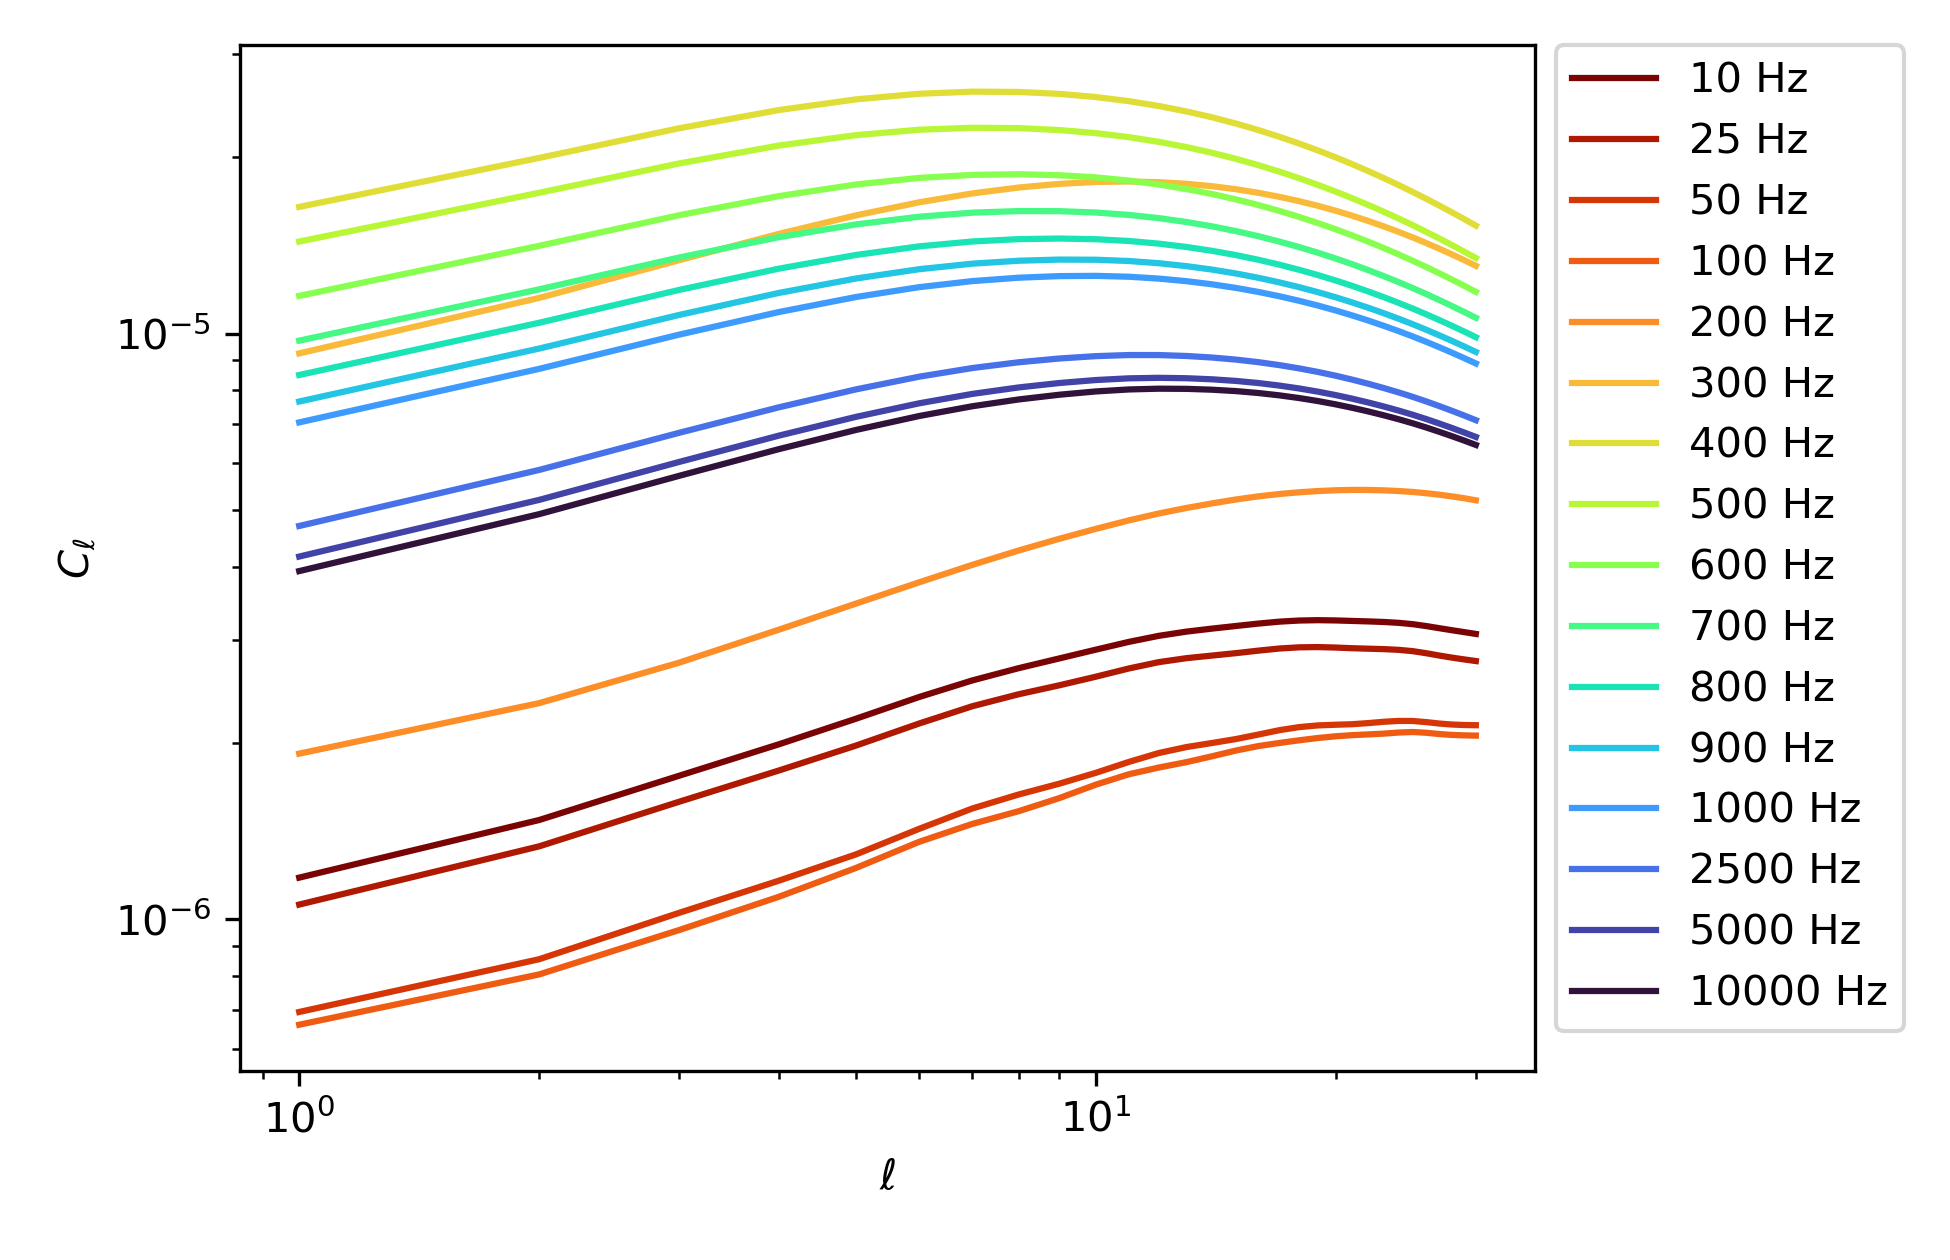
\includegraphics[width=1\linewidth]{Images/C_l_frequencies.png}
    \caption{AGWB angular power spectrum of different observed frequencies, going up to $l=30$.}
    \label{AGWB_anisotropies}
\end{figure} 

If we focus on the dipole $l=1$, we can plot it as a function of frequency, see Fig.\ref{dipole_1000Hz}.

\begin{figure}
    \centering
    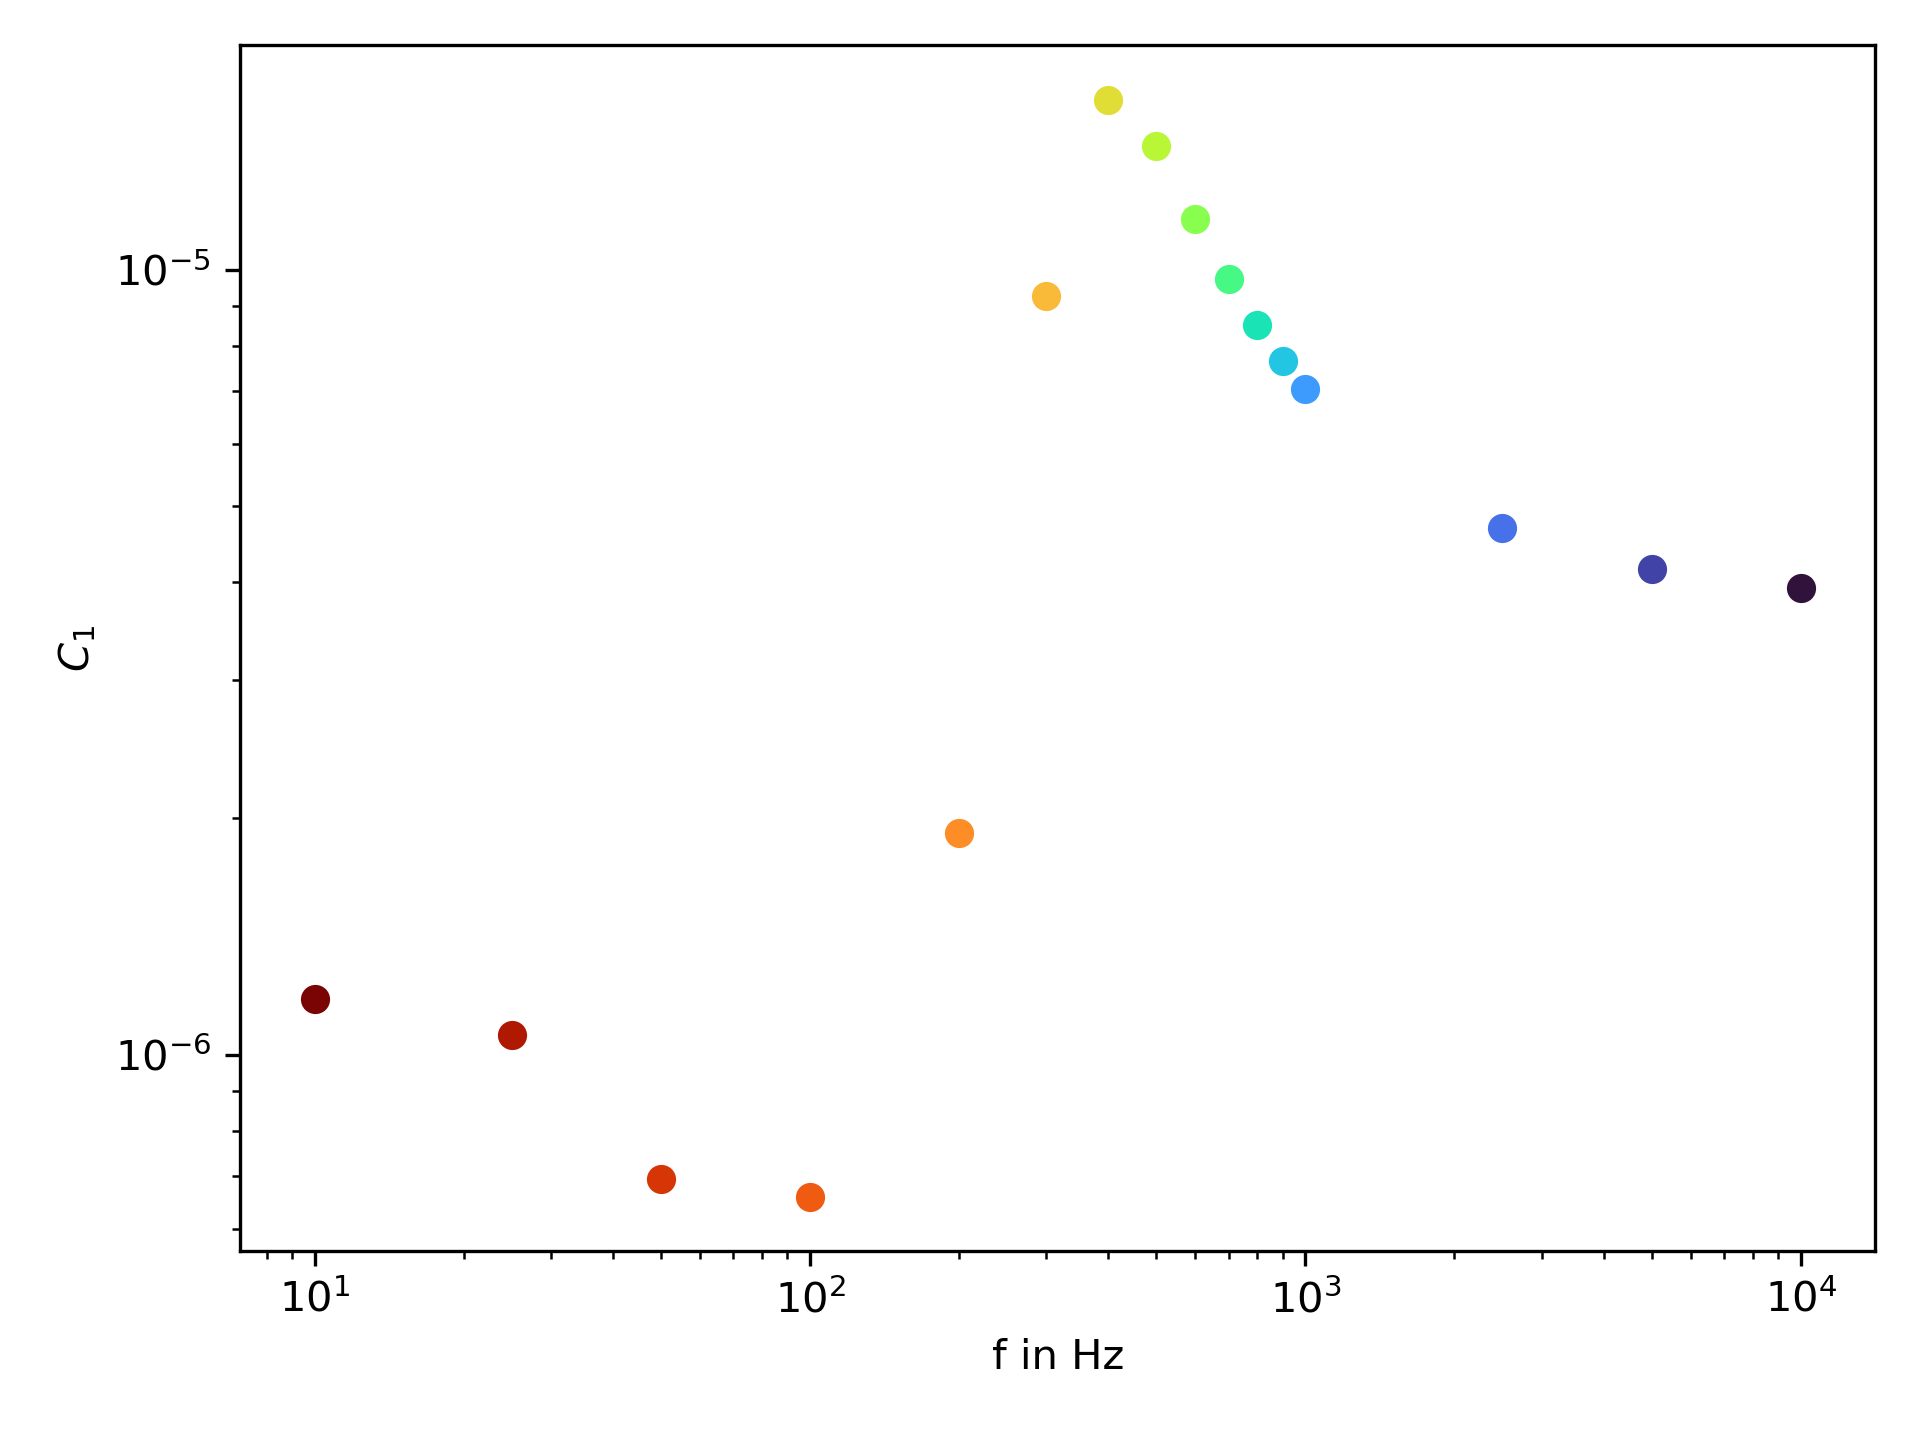
\includegraphics[width=0.8\linewidth]{Images/dipole_frequencies_10000Hz.png}
    \caption{The dipole of the AGWB at different observed frequencies.}
    \label{dipole_1000Hz}
\end{figure} 


\begin{figure}
    \centering
    \subfloat[{This work}
        \label{lorenzo_dipole}]{
        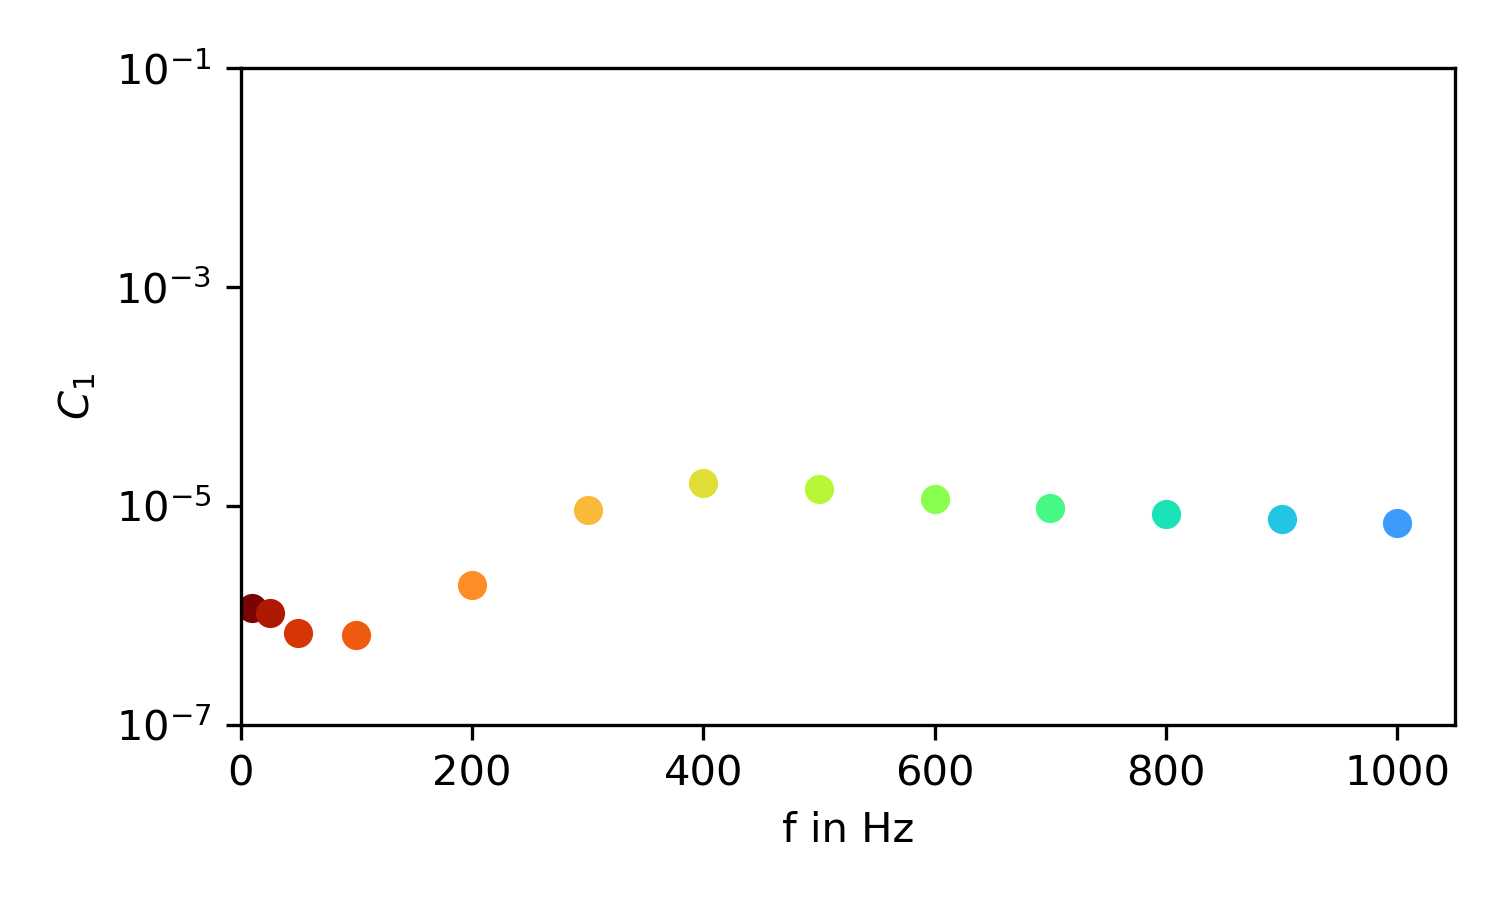
\includegraphics[width=8cm, clip]{Images/dipole_frequencies.png}}
    \subfloat[{\cite{dallarmi_dipole_2022}}
        \label{dipole_1000Hz}]{
        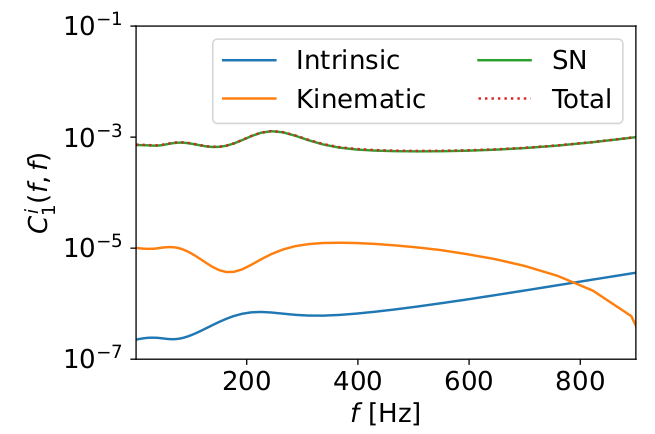
\includegraphics[width=7cm, clip]{Images/lorenzo_dipole.png}}
    \caption{Comparison of the computed dipole contribution to \cite{dallarmi_dipole_2022}. On the left are the computed anisotropies using our formalism for the intrinsic anisotropies. On the right, the computed dipole by \cite{dallarmi_dipole_2022}. The intrinsic dipole is shown in blue, the kinematic dipole in orange and the shot noise for the dipole in green.}
    \label{lorenzo_comparison}
\end{figure} 


\section{AGWB vs. Noise}


\subsection{1D Toy Model}

To show how {\tt NIFTy} works in principle, we will reconstruct a one-dimensional power spectrum. From this input, a random realisation of data points is drawn from which the signal is reconstructed. The reconstruction and the residual plot are shown in Fig. \ref{1D_reconstruction}.In this case, the reconstruction works quite well. 

\begin{figure}[h]
    \centering
    \subfloat{
        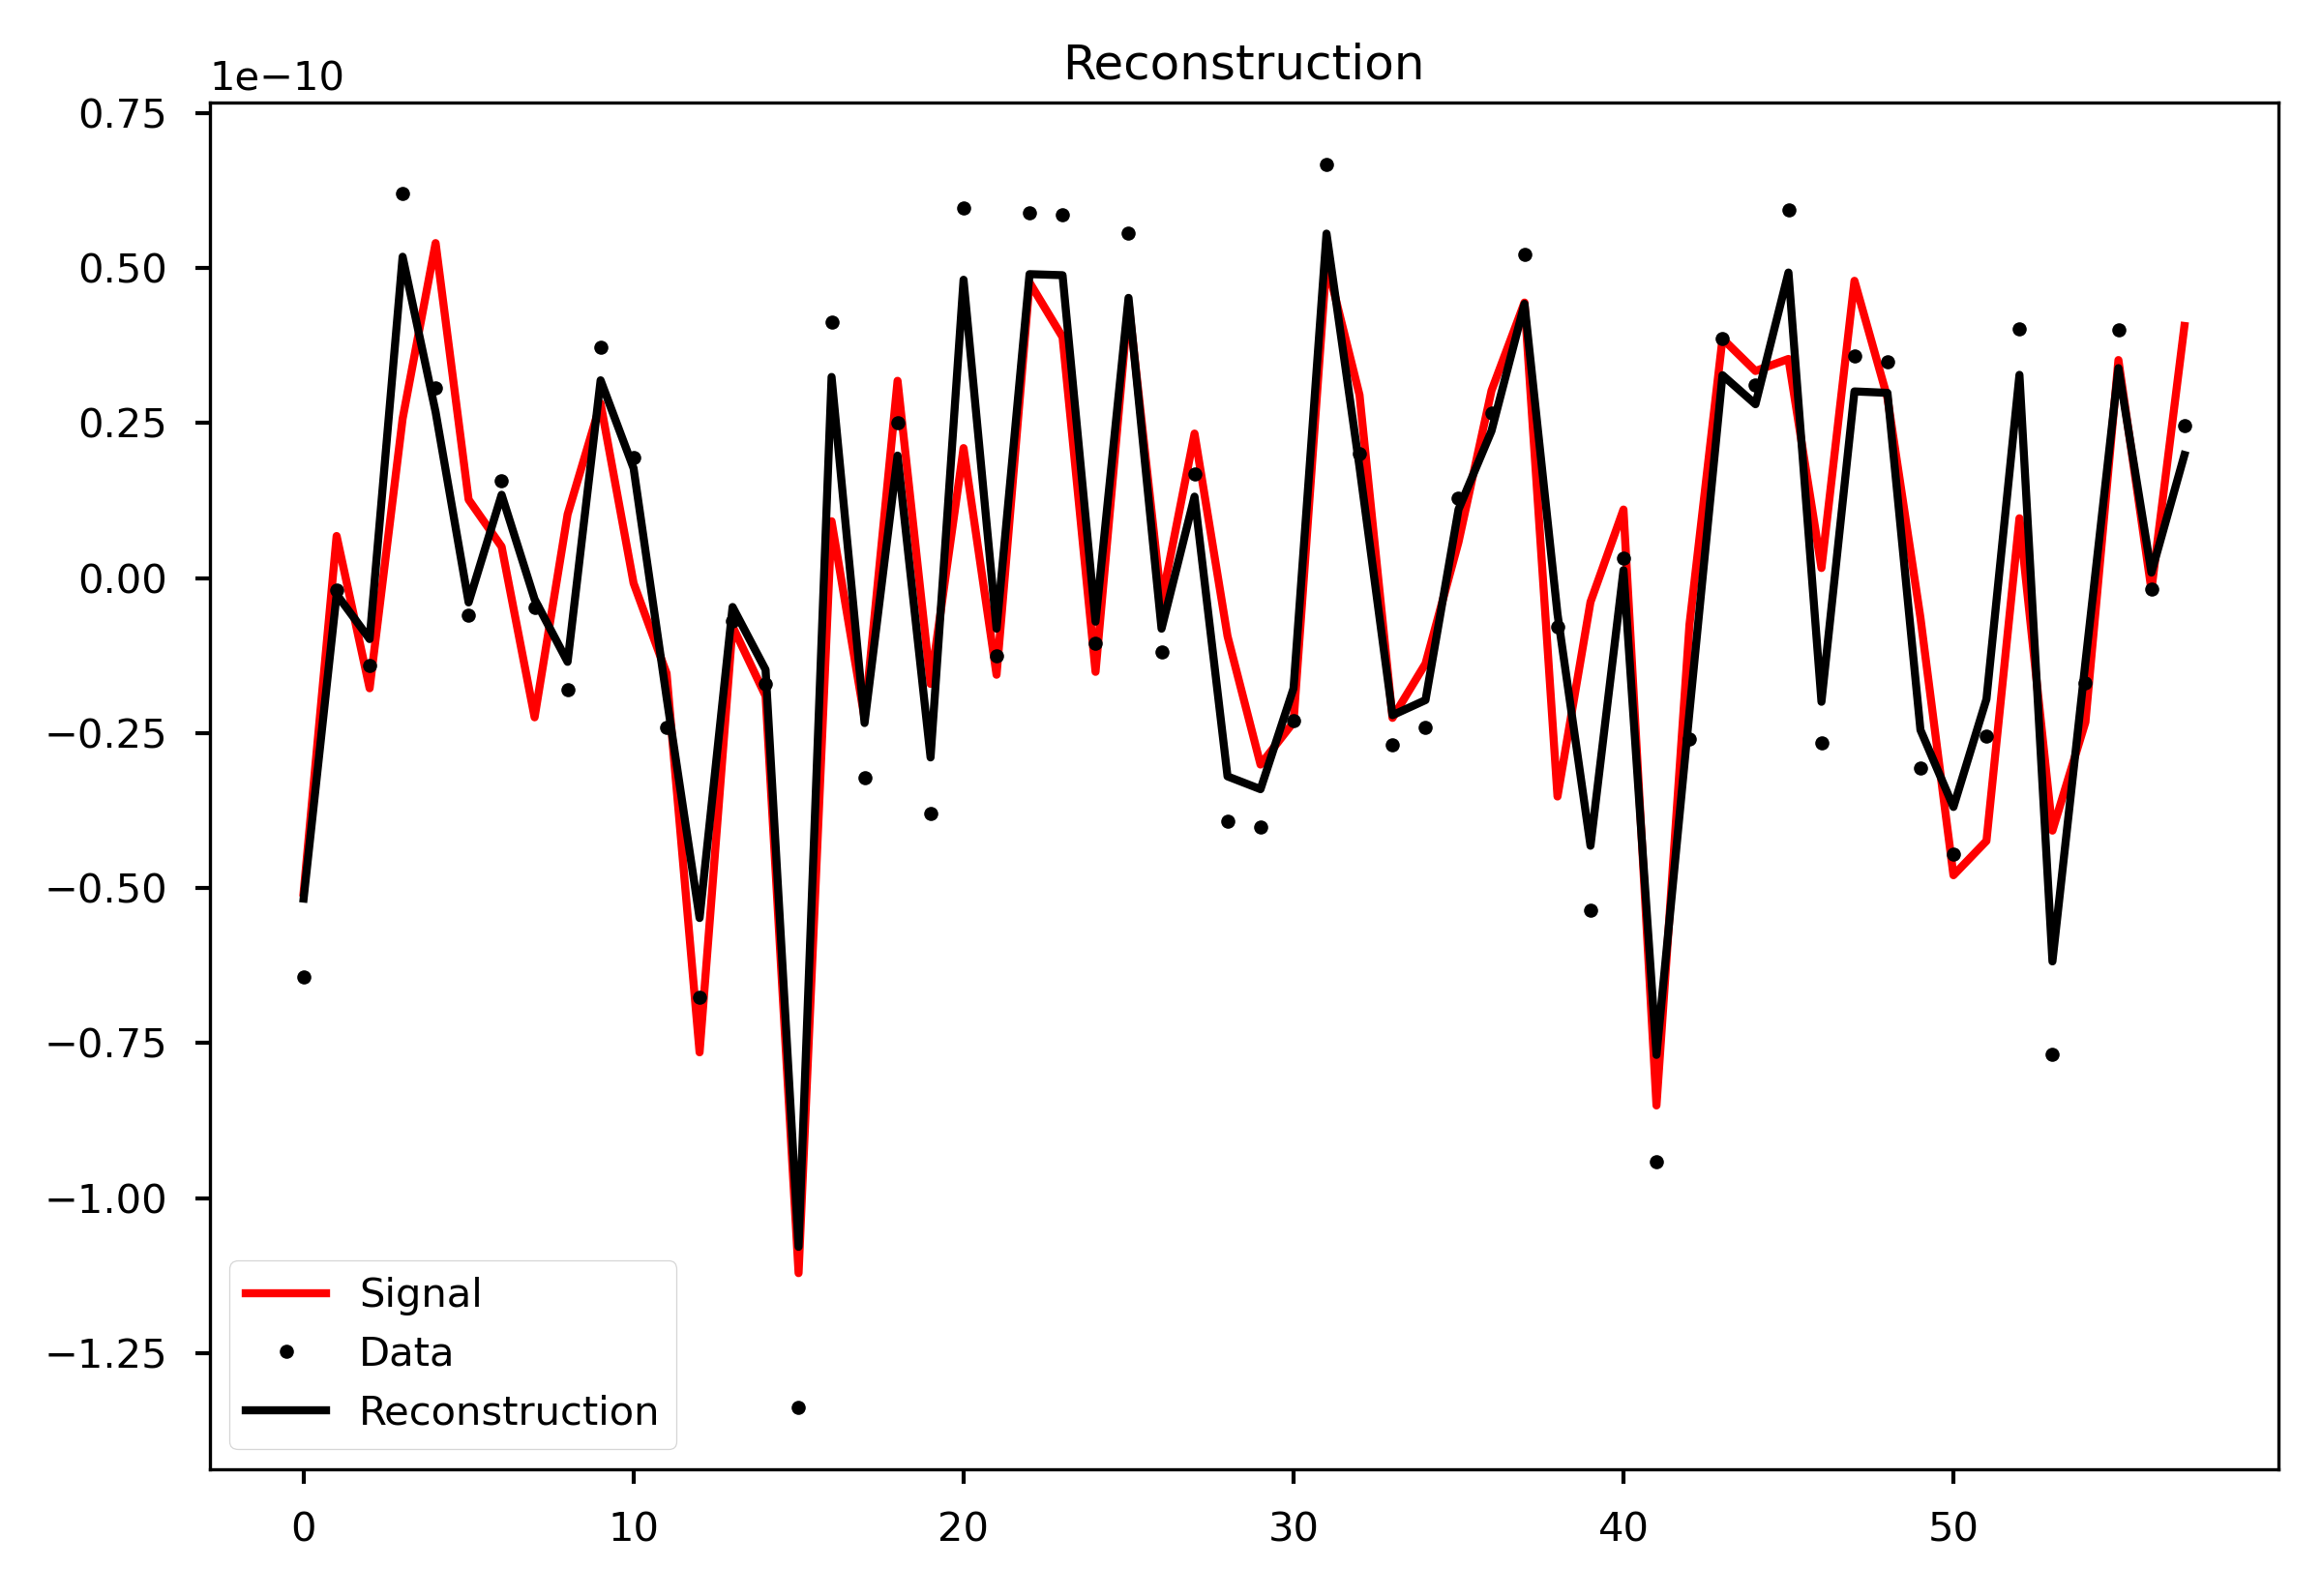
\includegraphics[width=7.5cm, clip]{Images/recon_400Hz_1D.png}}
    \subfloat{
        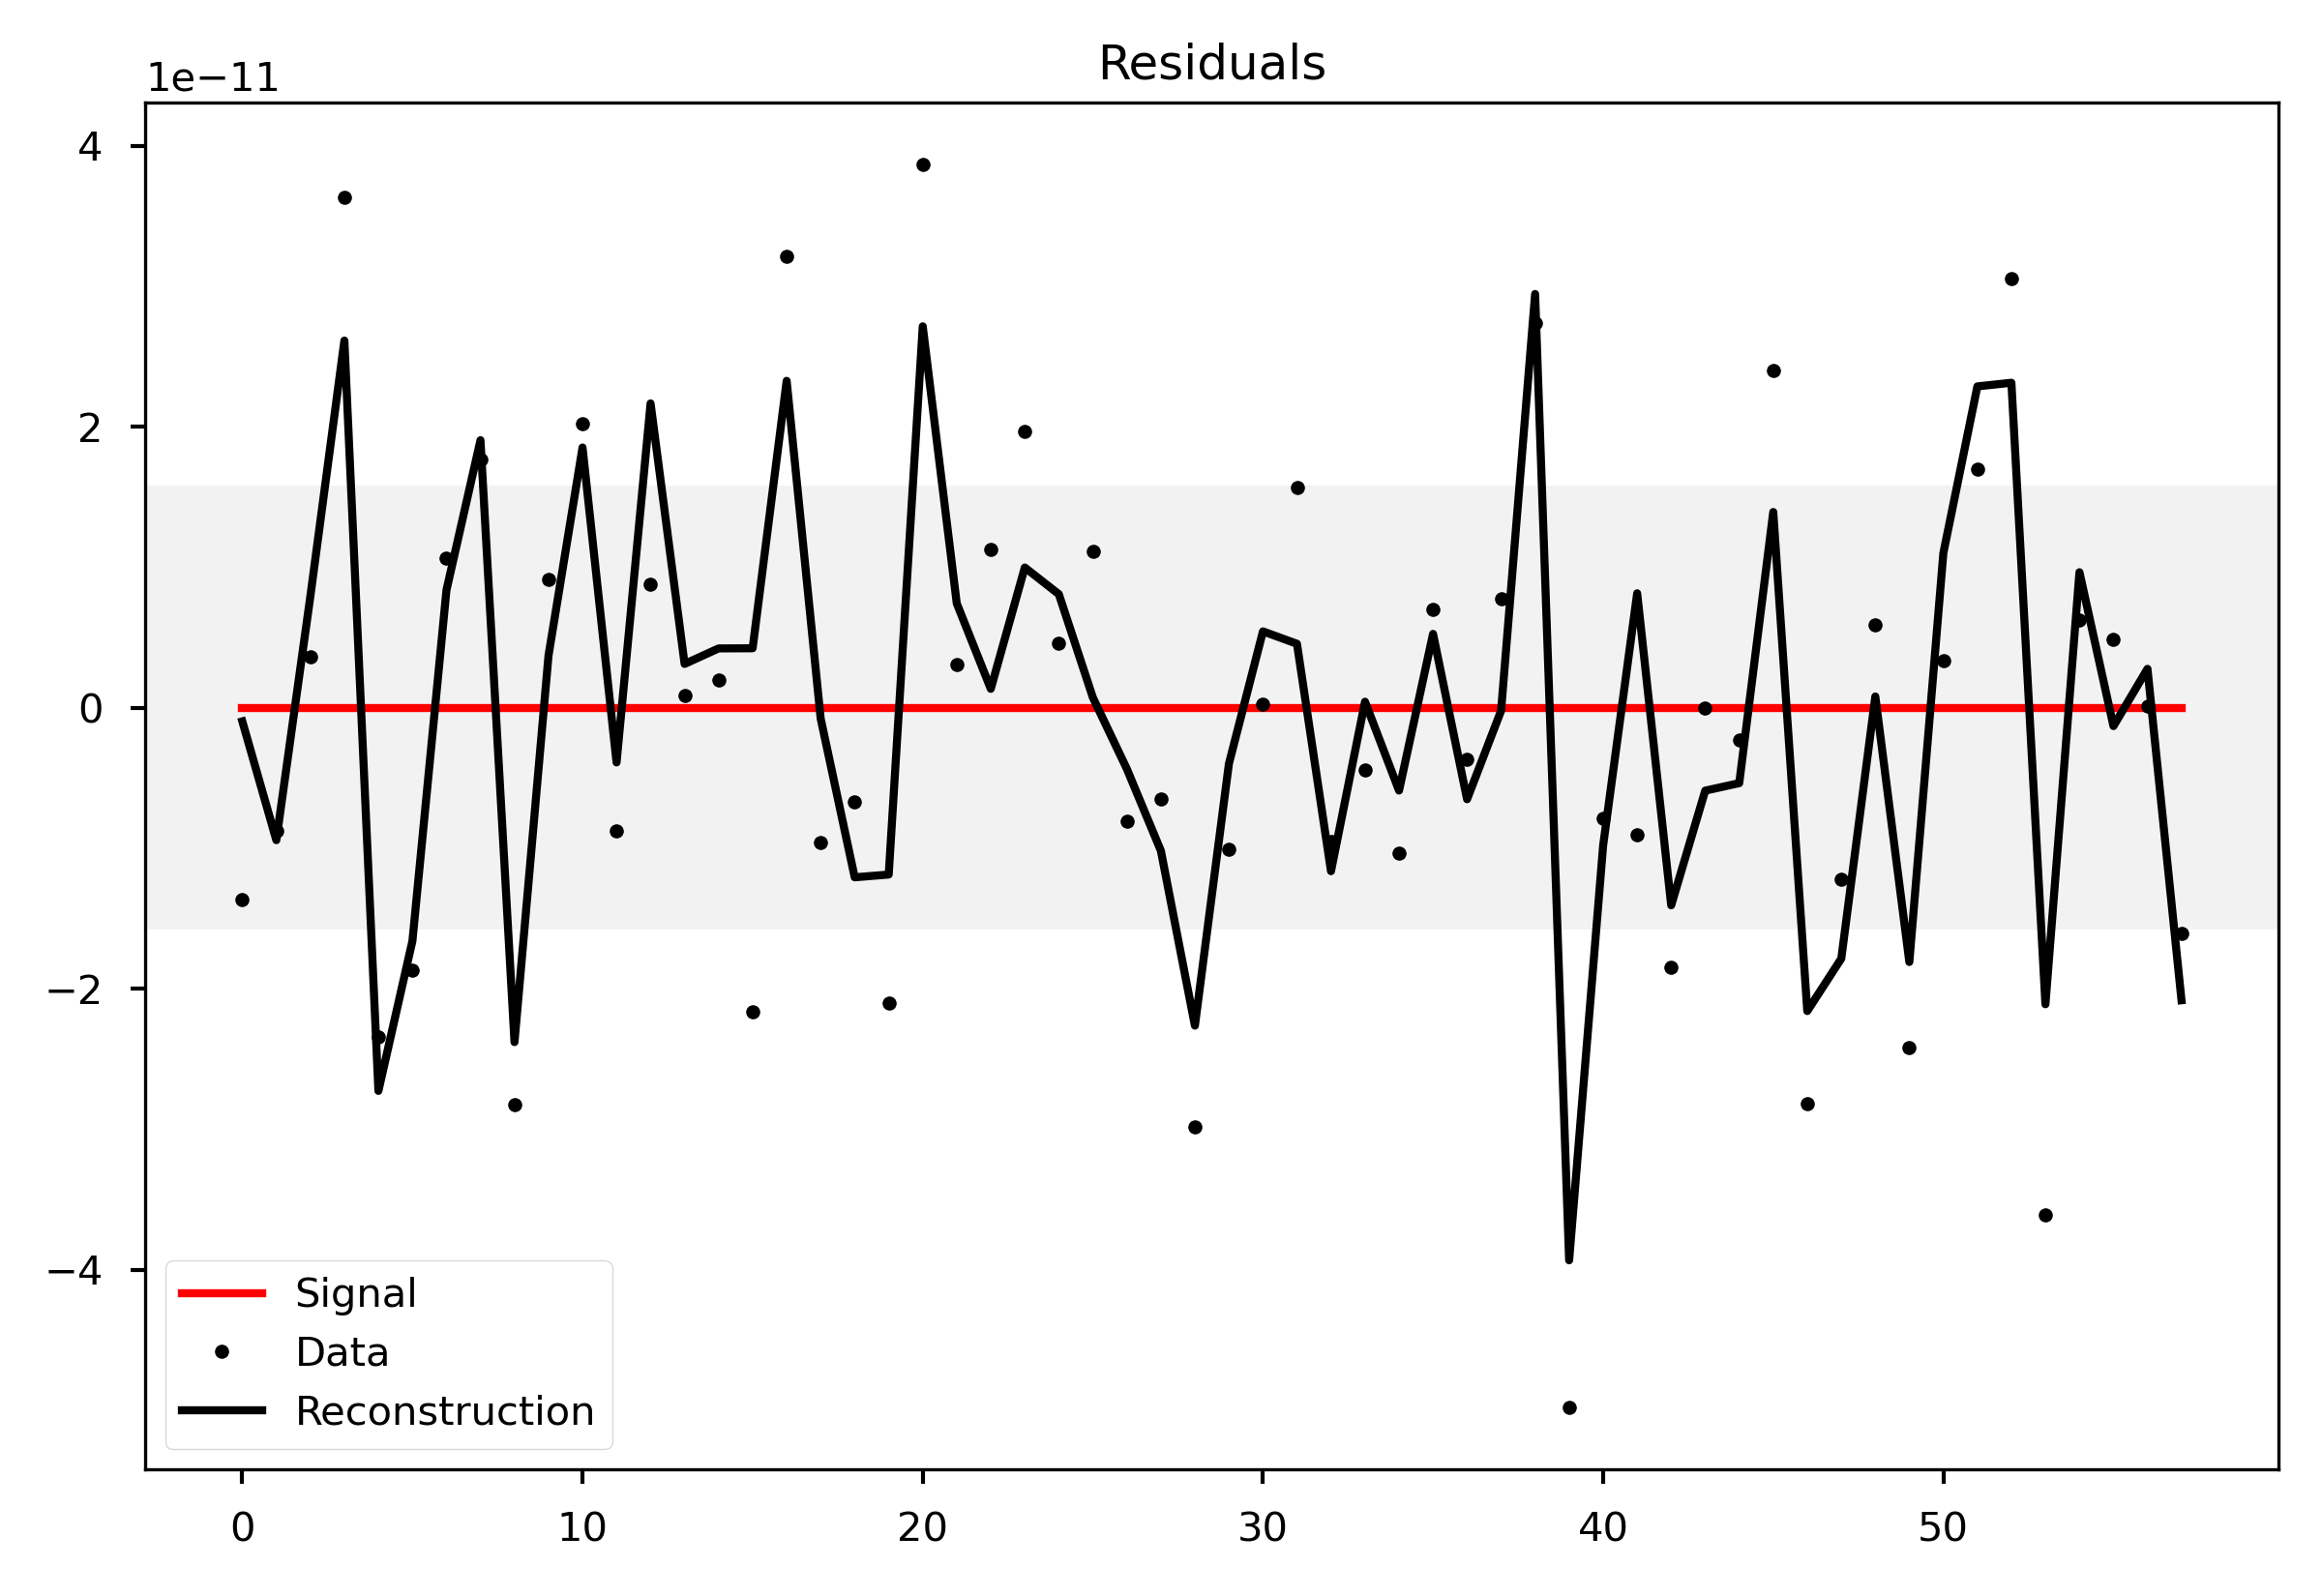
\includegraphics[width=7.5cm, clip]{Images/residuals_400Hz_1D.png}}
    \caption{An example of using the {\tt NIFTy} code to reconstruct the power spectrum computed in this work, but in one dimension.}
    \label{1D_reconstruction}
\end{figure}

\begin{figure}[h]
    \centering
    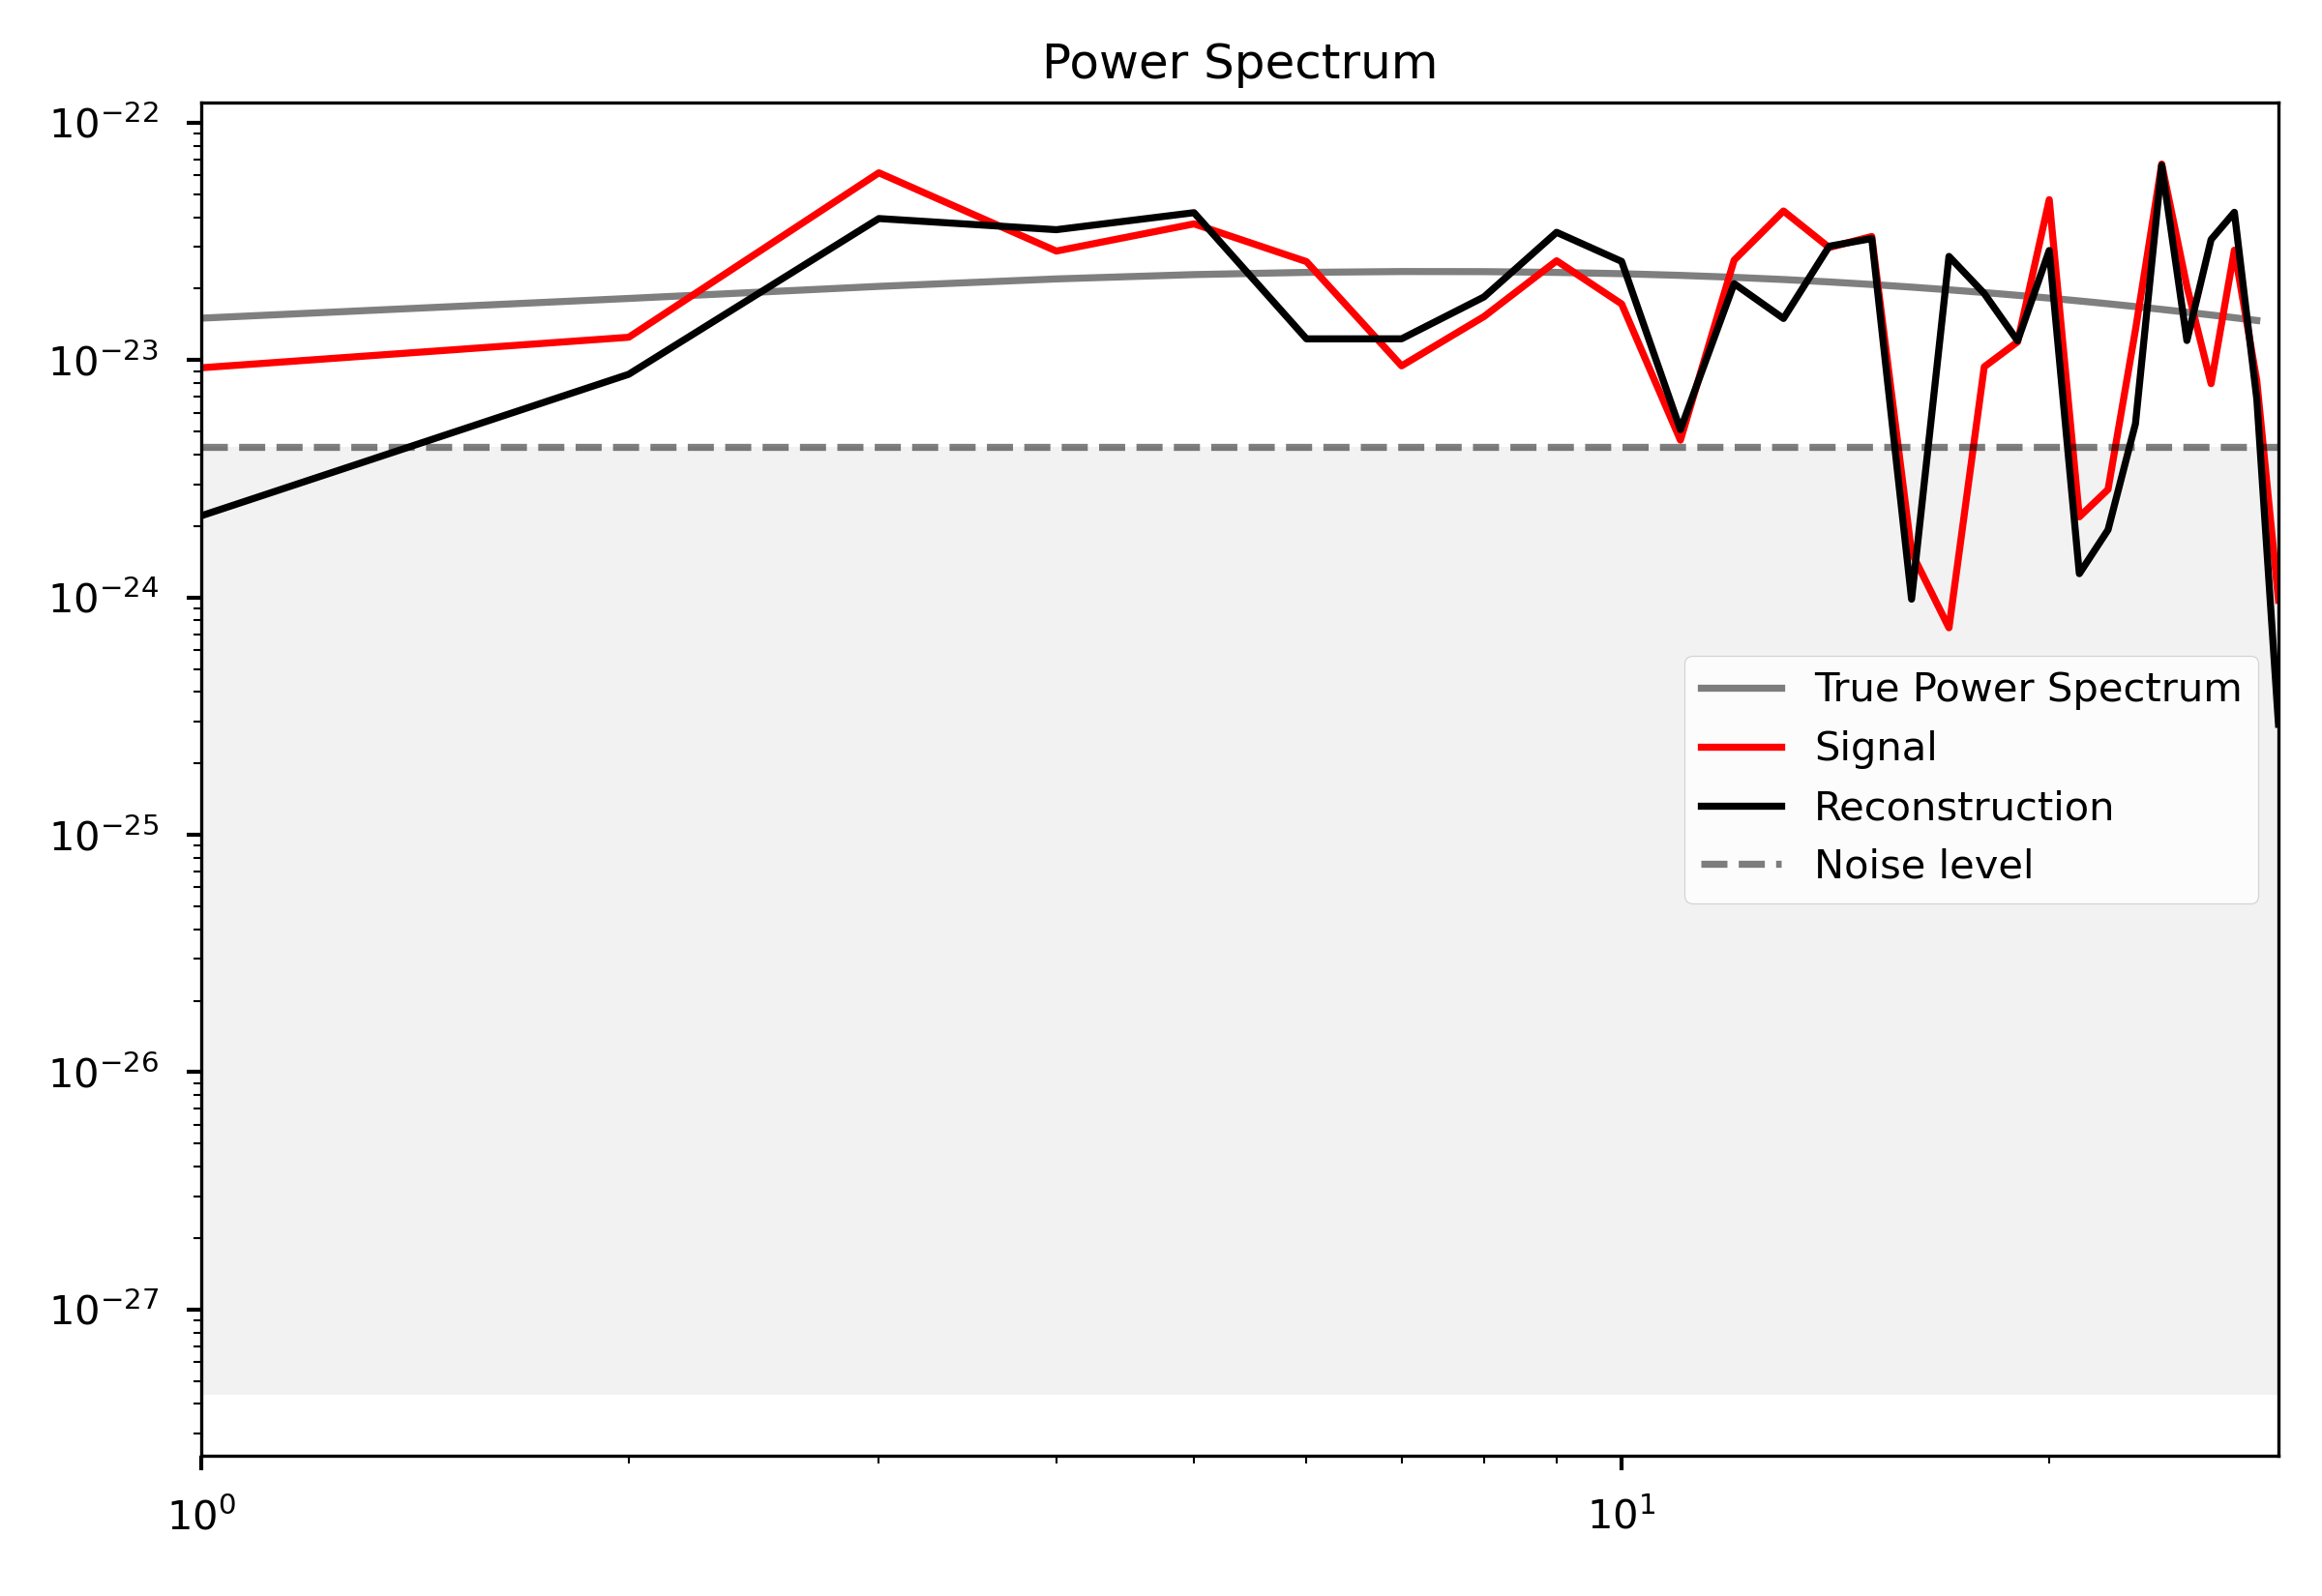
\includegraphics[width=0.8\linewidth]{Images/power_spectrum_400Hz_1D.png}
    \caption{The power spectra of the one-dimensional toy model. The input power spectrum is shown in grey, the signal realisation in red and the reconstruction using IFT in black.}
    \label{1D_power_spectrum}
\end{figure} 

In Fig.\ref{1D_power_spectrum}, we show different power spectra, i.e. the input, the one from the randomly drawn signal and the reconstruction. The reconstruction power spectrum is very similar to the signal one in this toy model.

\subsection{Sky Map}
\begin{figure}[h]
    \centering
    \subfloat{\hspace{0.75cm}
        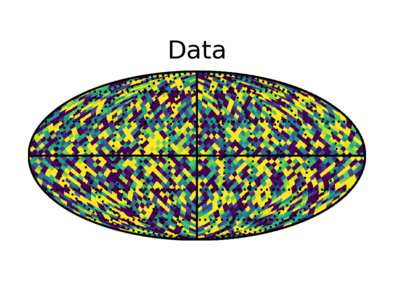
\includegraphics[width=6cm]{Images/data_100Hz_2D.png}
        }
    \newline
    \vspace{-1cm}
    \subfloat{
        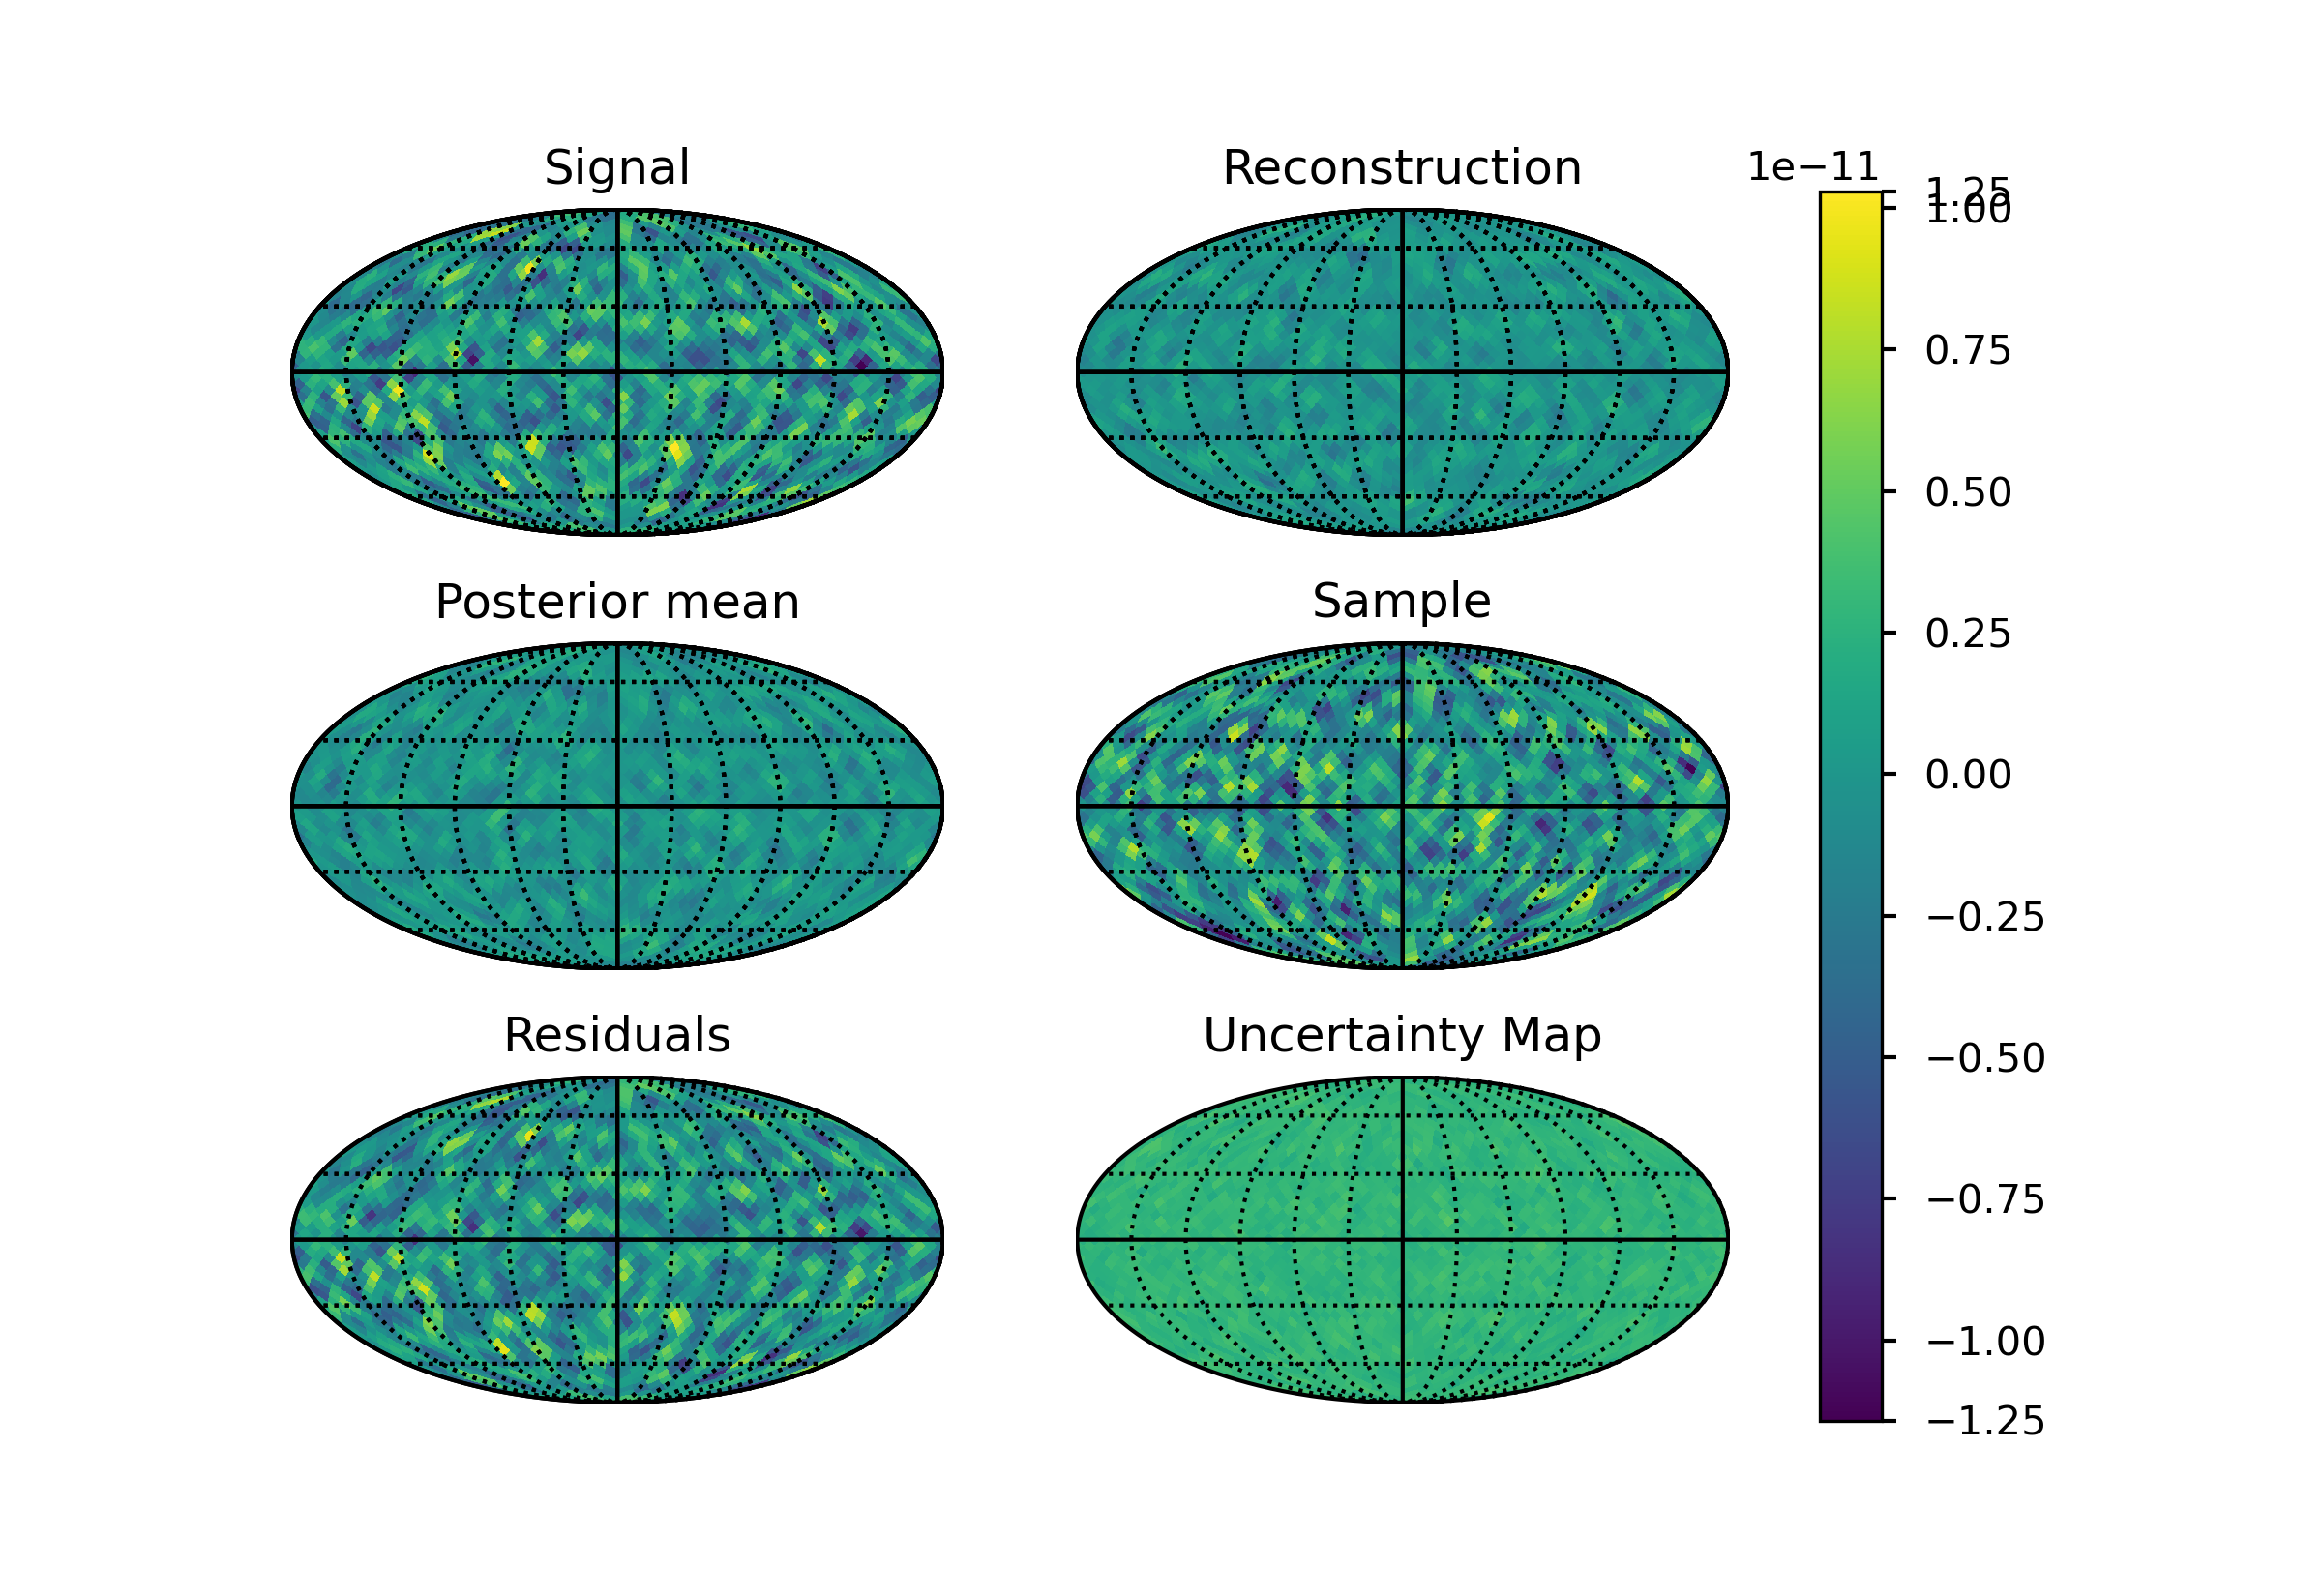
\includegraphics[width=\linewidth]{Images/6plot_100Hz_2D.png}}
    \caption{Reconstruction of the AGWB at 100 Hertz on a sky map using the {\tt NIFTy} code. The data on top is generated from the signal which is a realisation of the input power spectrum. The posterior mean is calculated using a Wiener filter. A sample of this is drawn randomly. The residuals represent the difference between signal and reconstruction from the first row. The uncertainty map shows the calculated errors on the reconstruction.}
    \label{sky_maps_100}
\end{figure}

\begin{figure}[h]
    \centering
    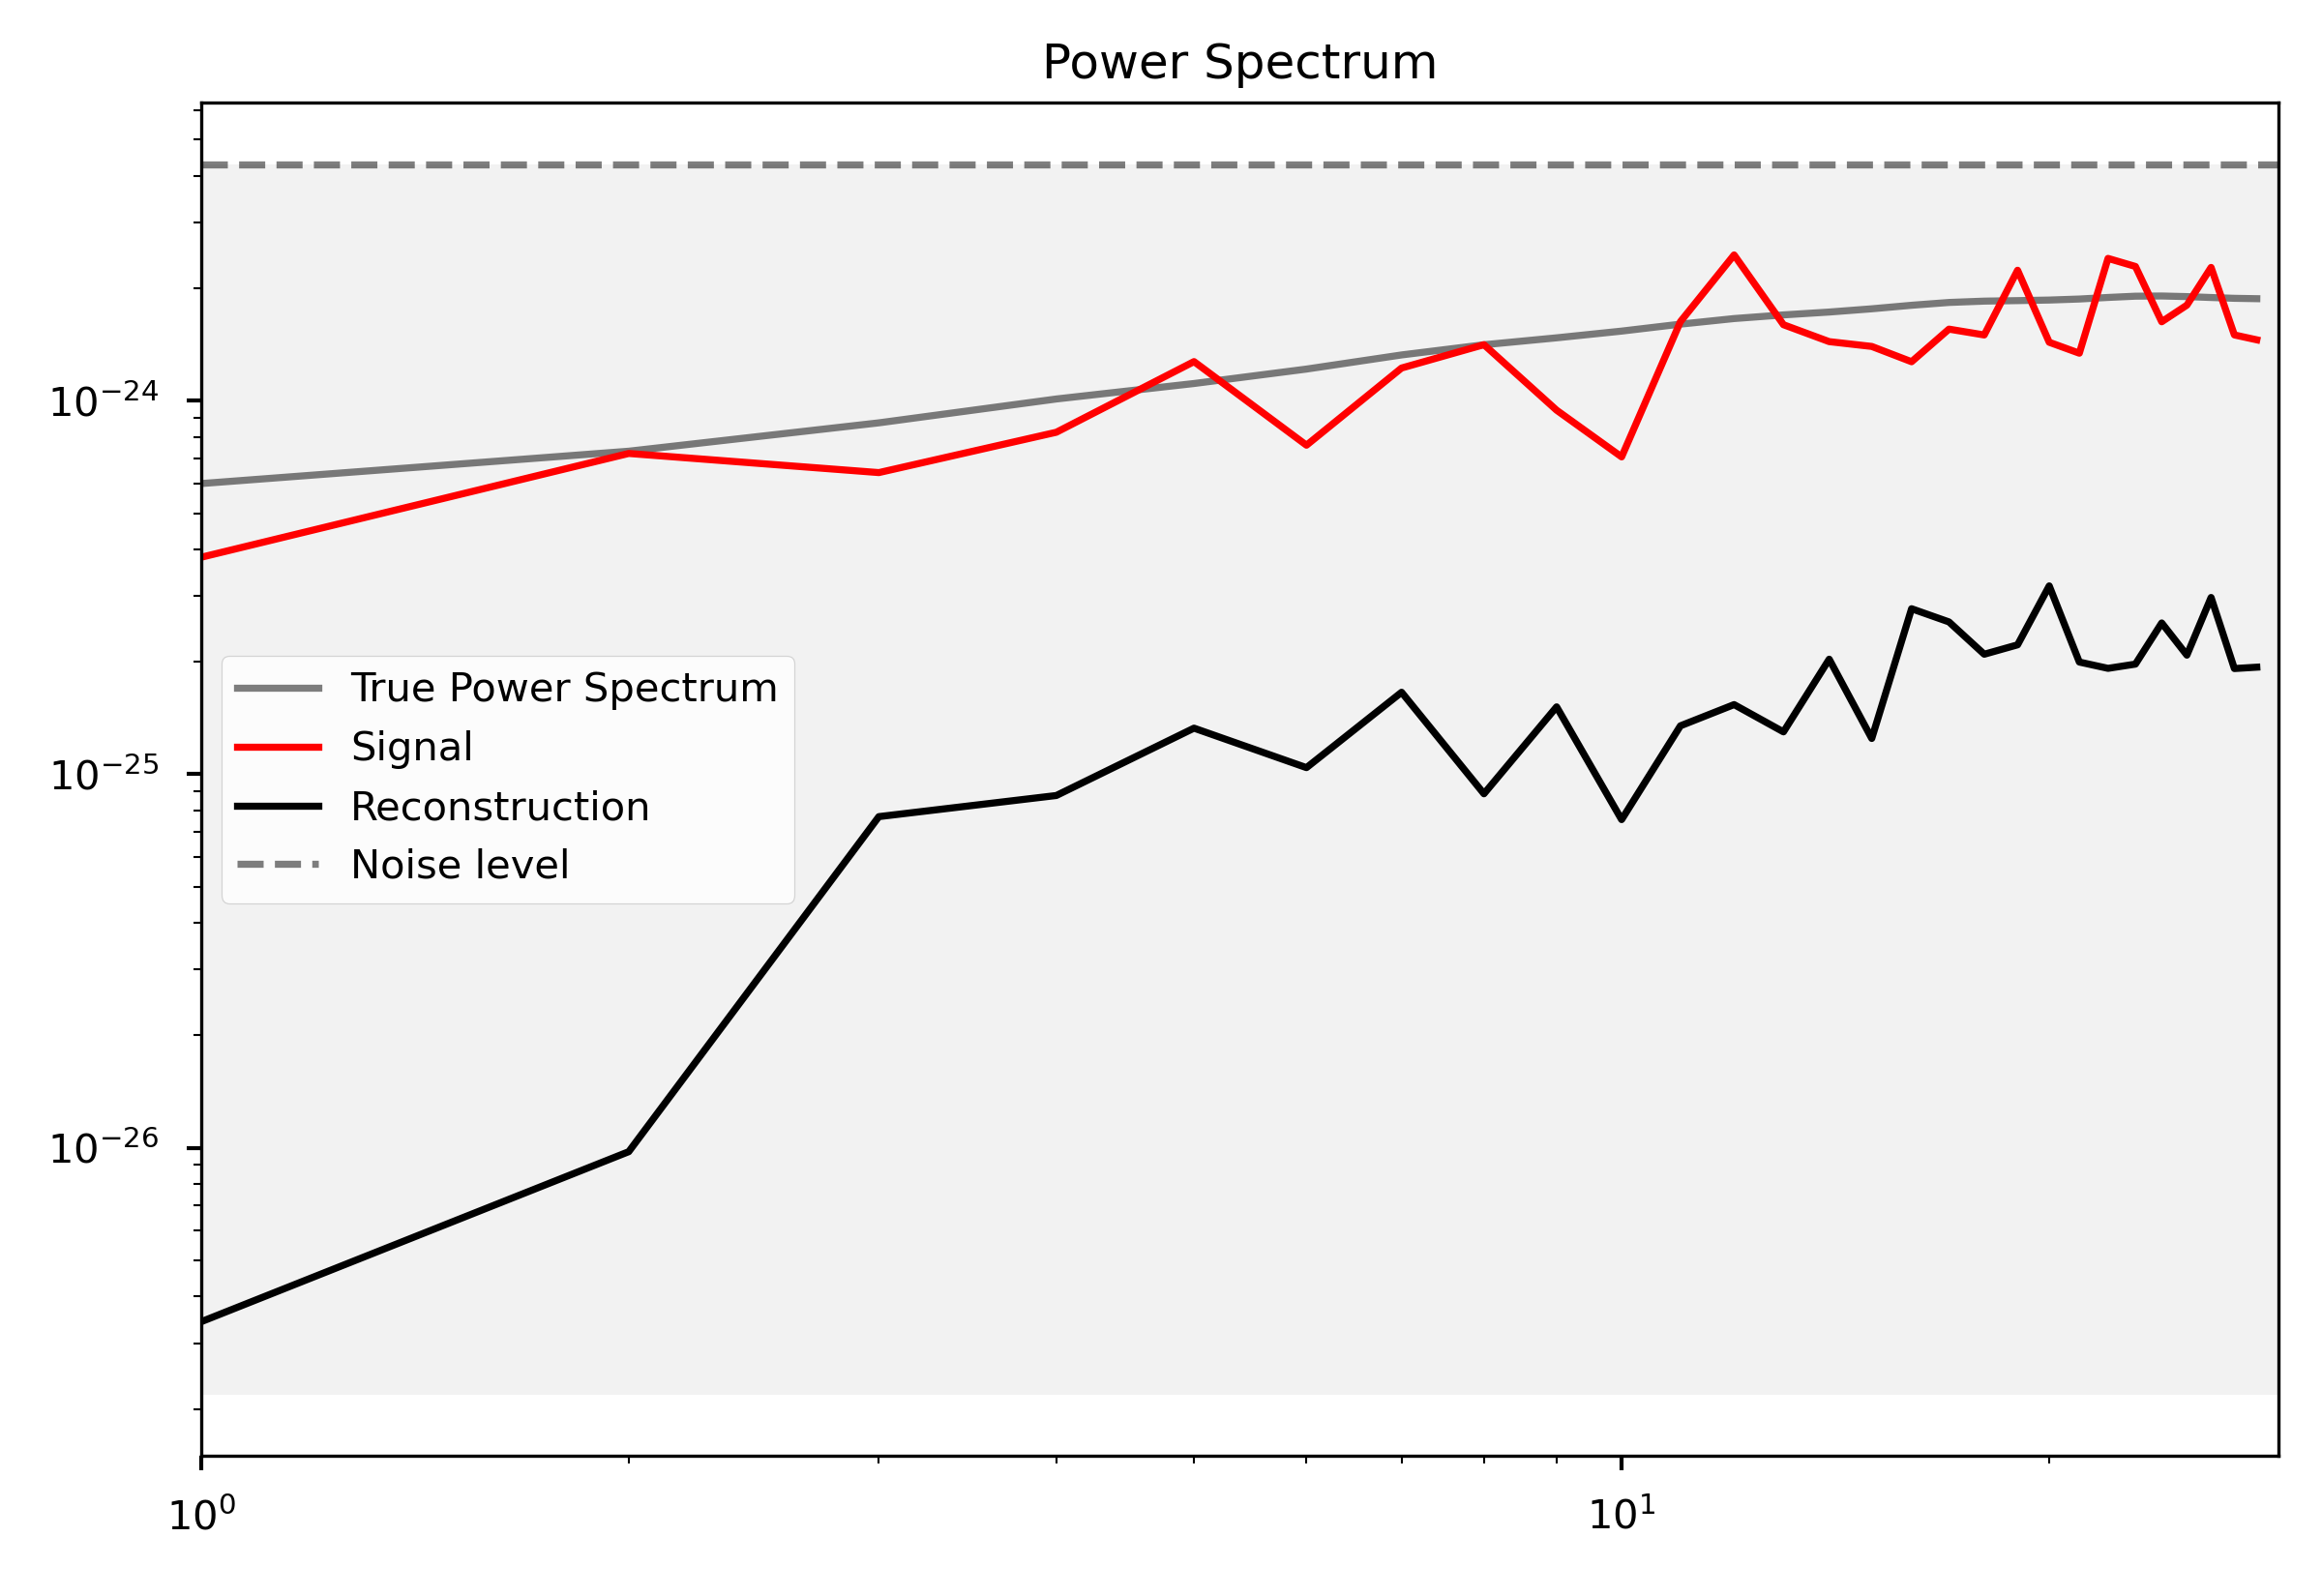
\includegraphics[width=0.8\linewidth]{Images/power_spectrum_100Hz_2D.png}
    \caption{The power spectra of the AGWB separation at 100 Hertz. The input power spectrum is shown in grey, the signal realisation in red and the reconstruction using IFT in black.}
    \label{100Hz_power_spectrum}
\end{figure} 

For the noise angular power spectrum, we assume Gaussian noise using the best anisotropic noise sensitivity for ET and CE using cross-correlations (at $l=1$). This is an optimistic assumption. The computed $C_l$ used for the separation reach up to $l=30$. Looking at Fig. \ref{ET_Cl}, our assumed noise curve would have the shape of $l+\frac{1}{2}$ up to $l=30$, which would increase more slowly than the actual sensitivity curve. 

As seen in Fig.\ref{AGWB_anisotropies}, we compute the lowest angular power spectrum at a frequency of 100 Hertz. To test the separation in this case, we use it as input for a reconstruction on a sky map using {\tt HEALPix}\cite{todo, healpix}. At this frequency, the separation is not successful. We see that the noise in the data in Fig.\ref{sky_maps_100} is higher than the original signal. The posterior mean and the reconstruction are both close to zero. Thus, the sample also does not mimick the signal and the residuals have the same order of magnitude as the original signal.


The AGWB has the highest angular power spectrum at 400 Hertz in our calculation (see Fig.\ref{AGWB_anisotropies}). So, we use this frequency to perform another IFT separation.

\begin{figure}[h]
    \centering
    \subfloat{\hspace{0.75cm}
        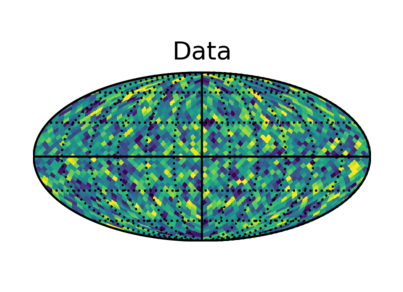
\includegraphics[width=6cm]{Images/data_400Hz_2D.png}
        }
    \newline
    \vspace{-1cm}
    \subfloat{
        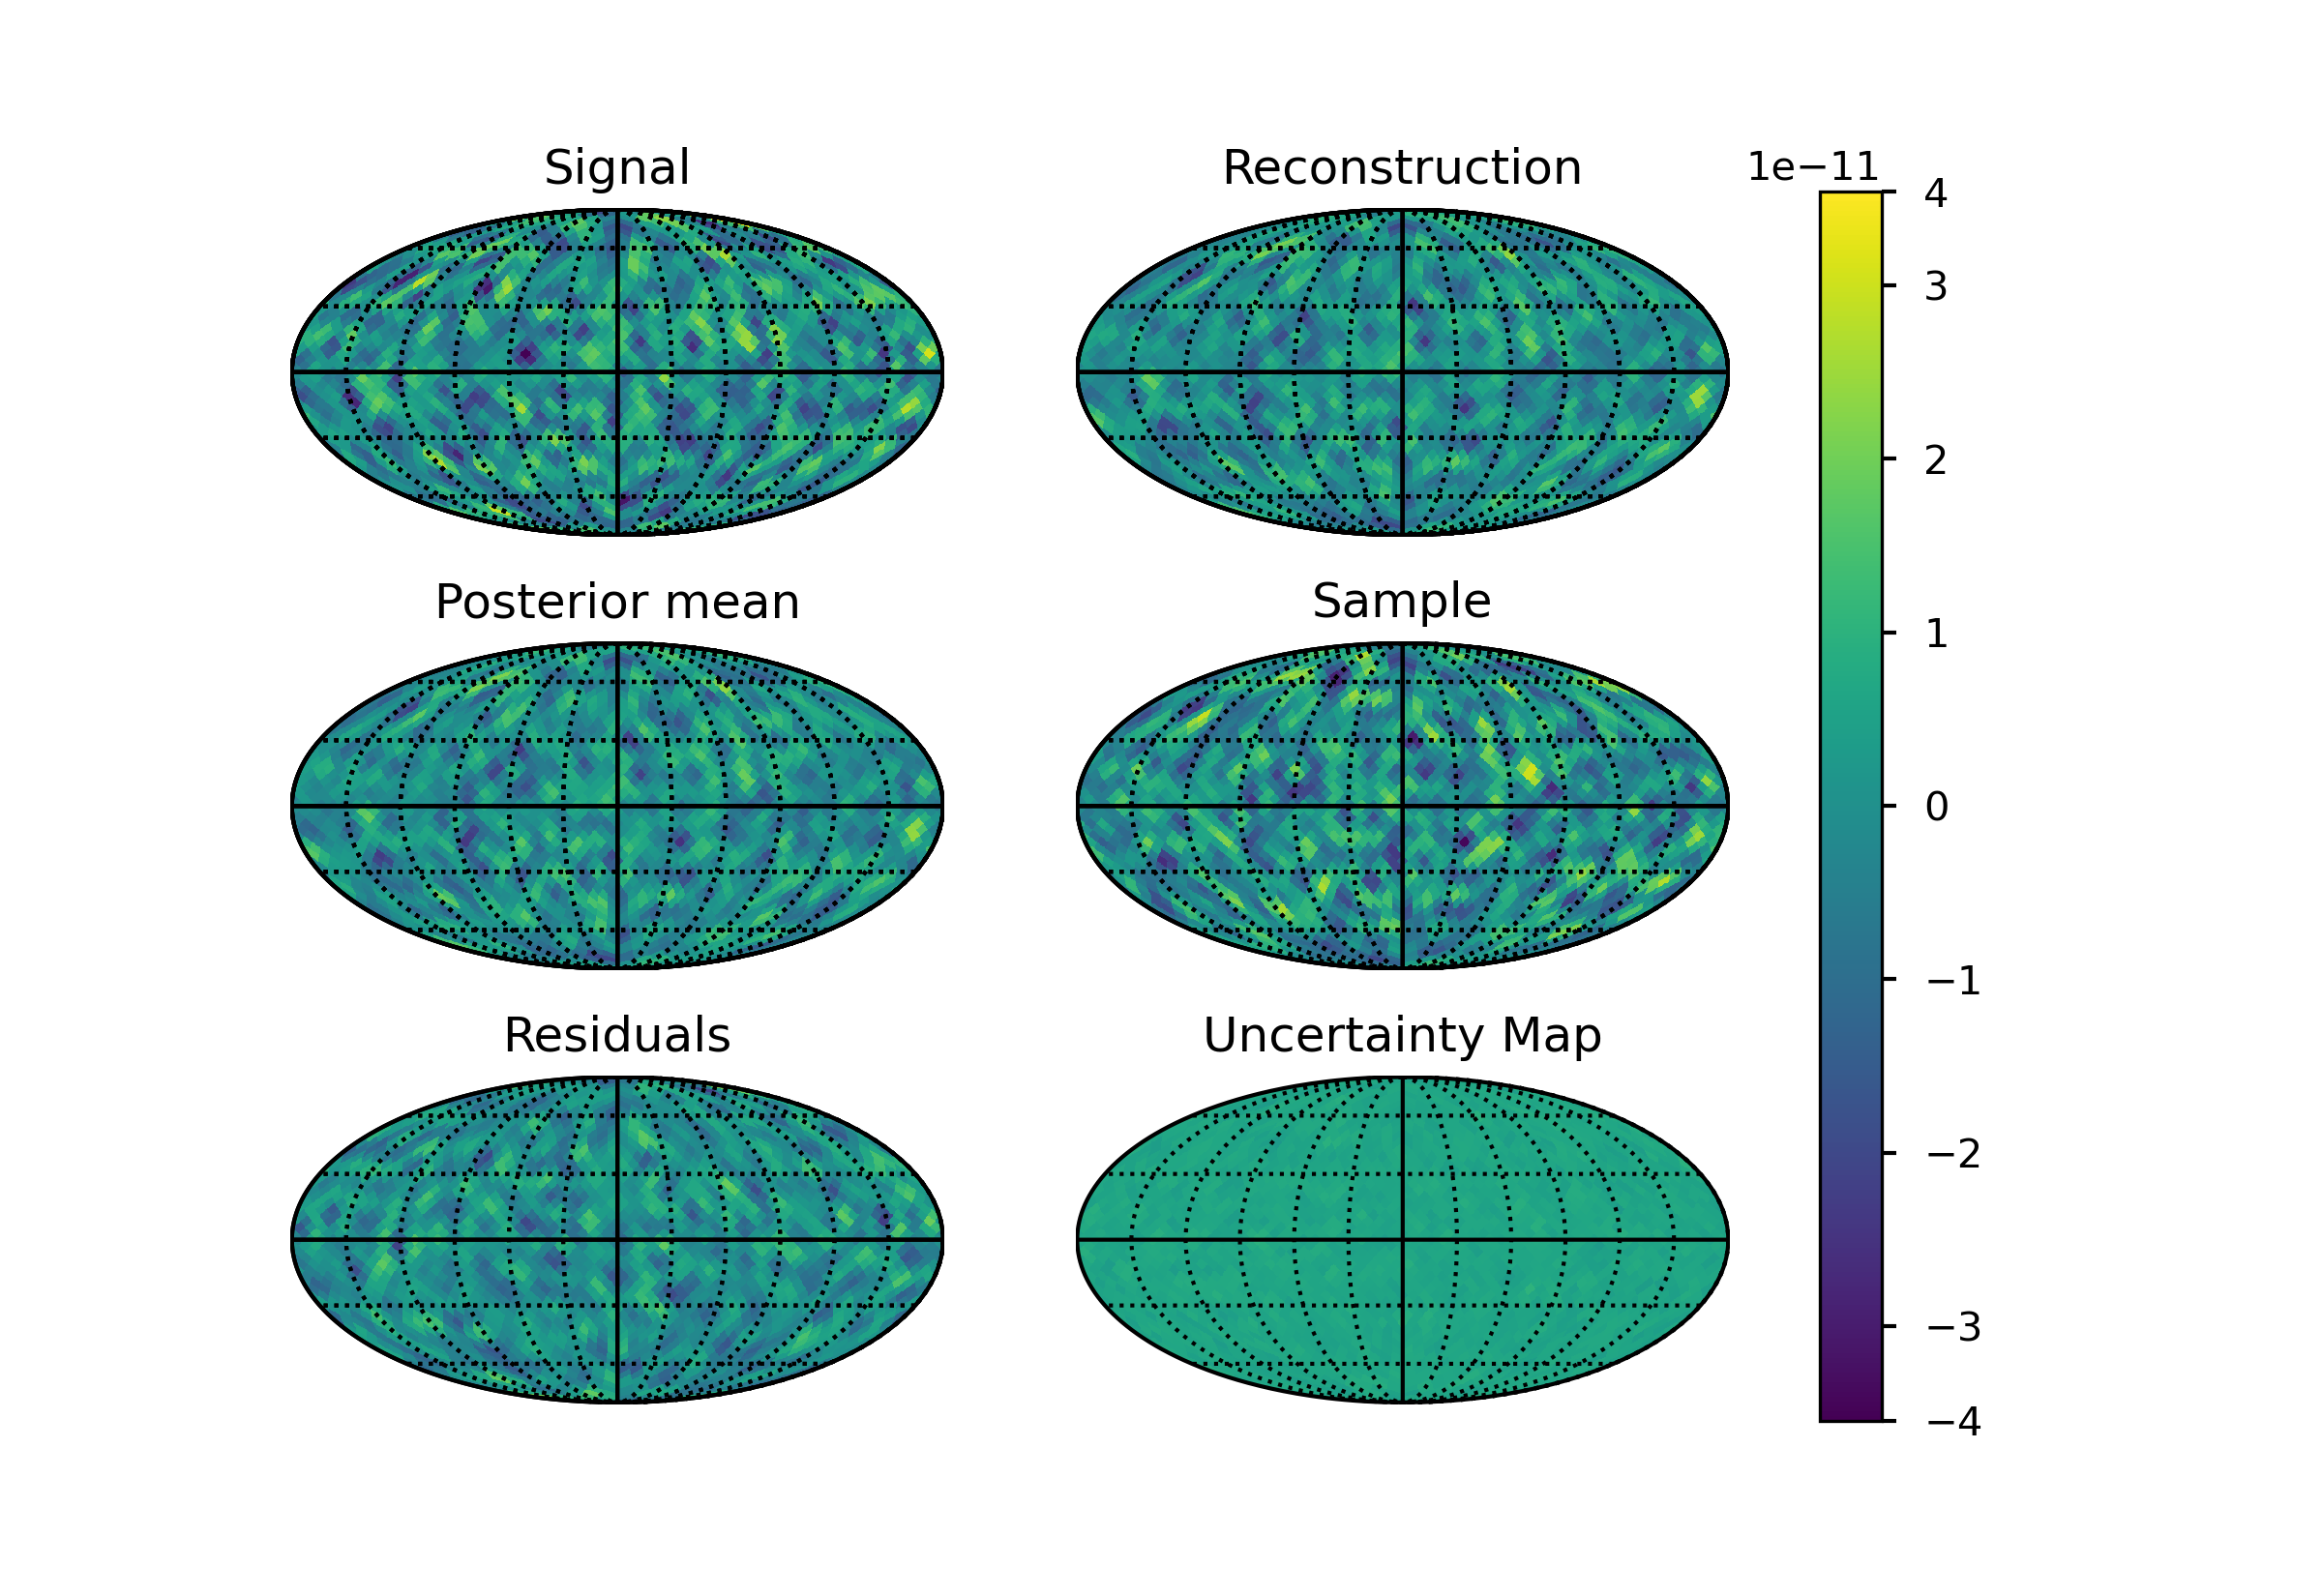
\includegraphics[width=\linewidth]{Images/6plot_400Hz_2D.png}}
    \caption{Reconstruction of the AGWB at 400 Hertz on a sky map using the {\tt NIFTy} code. The data on top is generated from the signal which is a realisation of the input power spectrum. The posterior mean is calculated using a Wiener filter. A sample of this is drawn randomly. The residuals represent the difference between signal and reconstruction from the first row. The uncertainty map shows the calculated errors on the reconstruction.}
    \label{sky_maps_400}
\end{figure}

\begin{figure}[h]
    \centering
    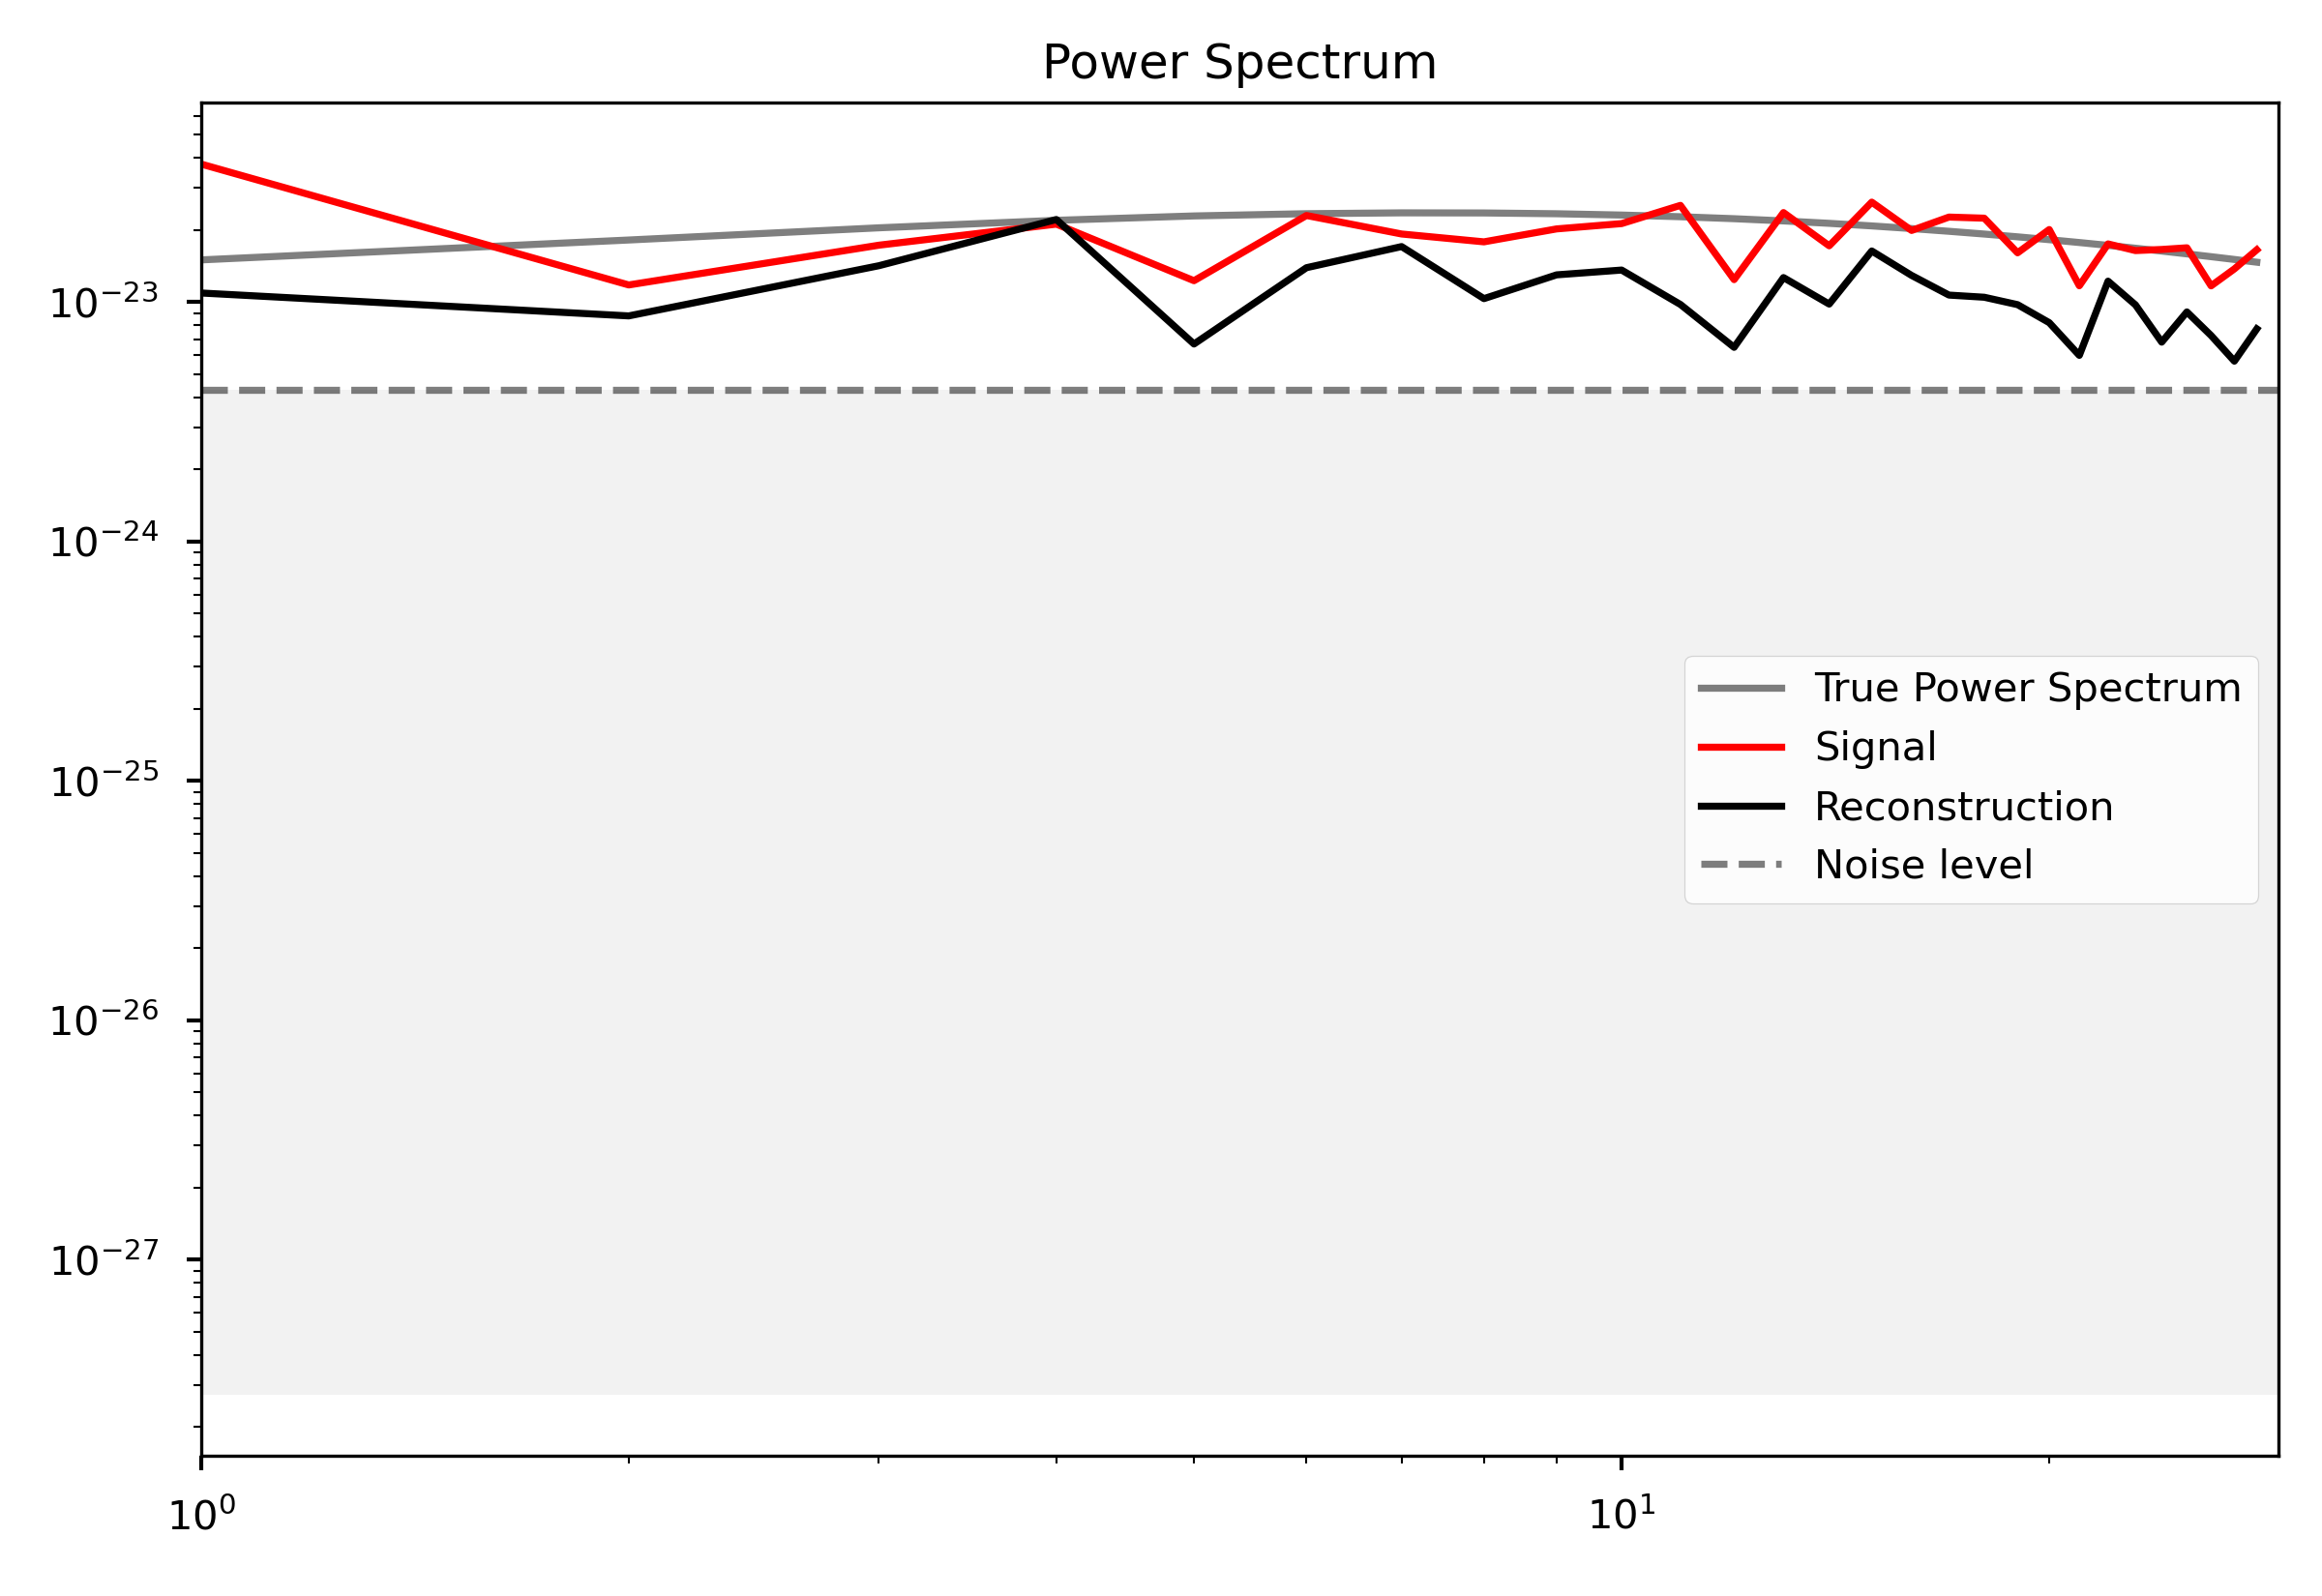
\includegraphics[width=0.8\linewidth]{Images/power_spectrum_400Hz_2D.png}
    \caption{The power spectra of the AGWB separation at 400 Hertz. The input power spectrum is shown in grey, the signal realisation in red and the reconstruction using IFT in black.}
    \label{400Hz_power_spectrum}
\end{figure} 

\section{CGWB vs. Noise}
\subsection{Sky Map}

\begin{figure}[h]
    \centering
    \subfloat{\hspace{0.75cm}
        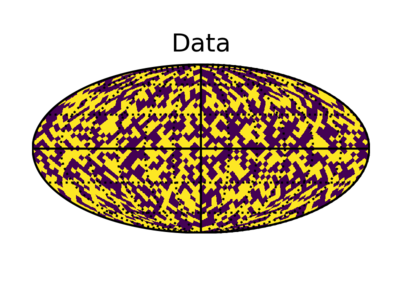
\includegraphics[width=6cm]{Images/data_cosmo_900Hz_2D.png}
        }
    \newline
    \vspace{-1cm}
    \subfloat{
        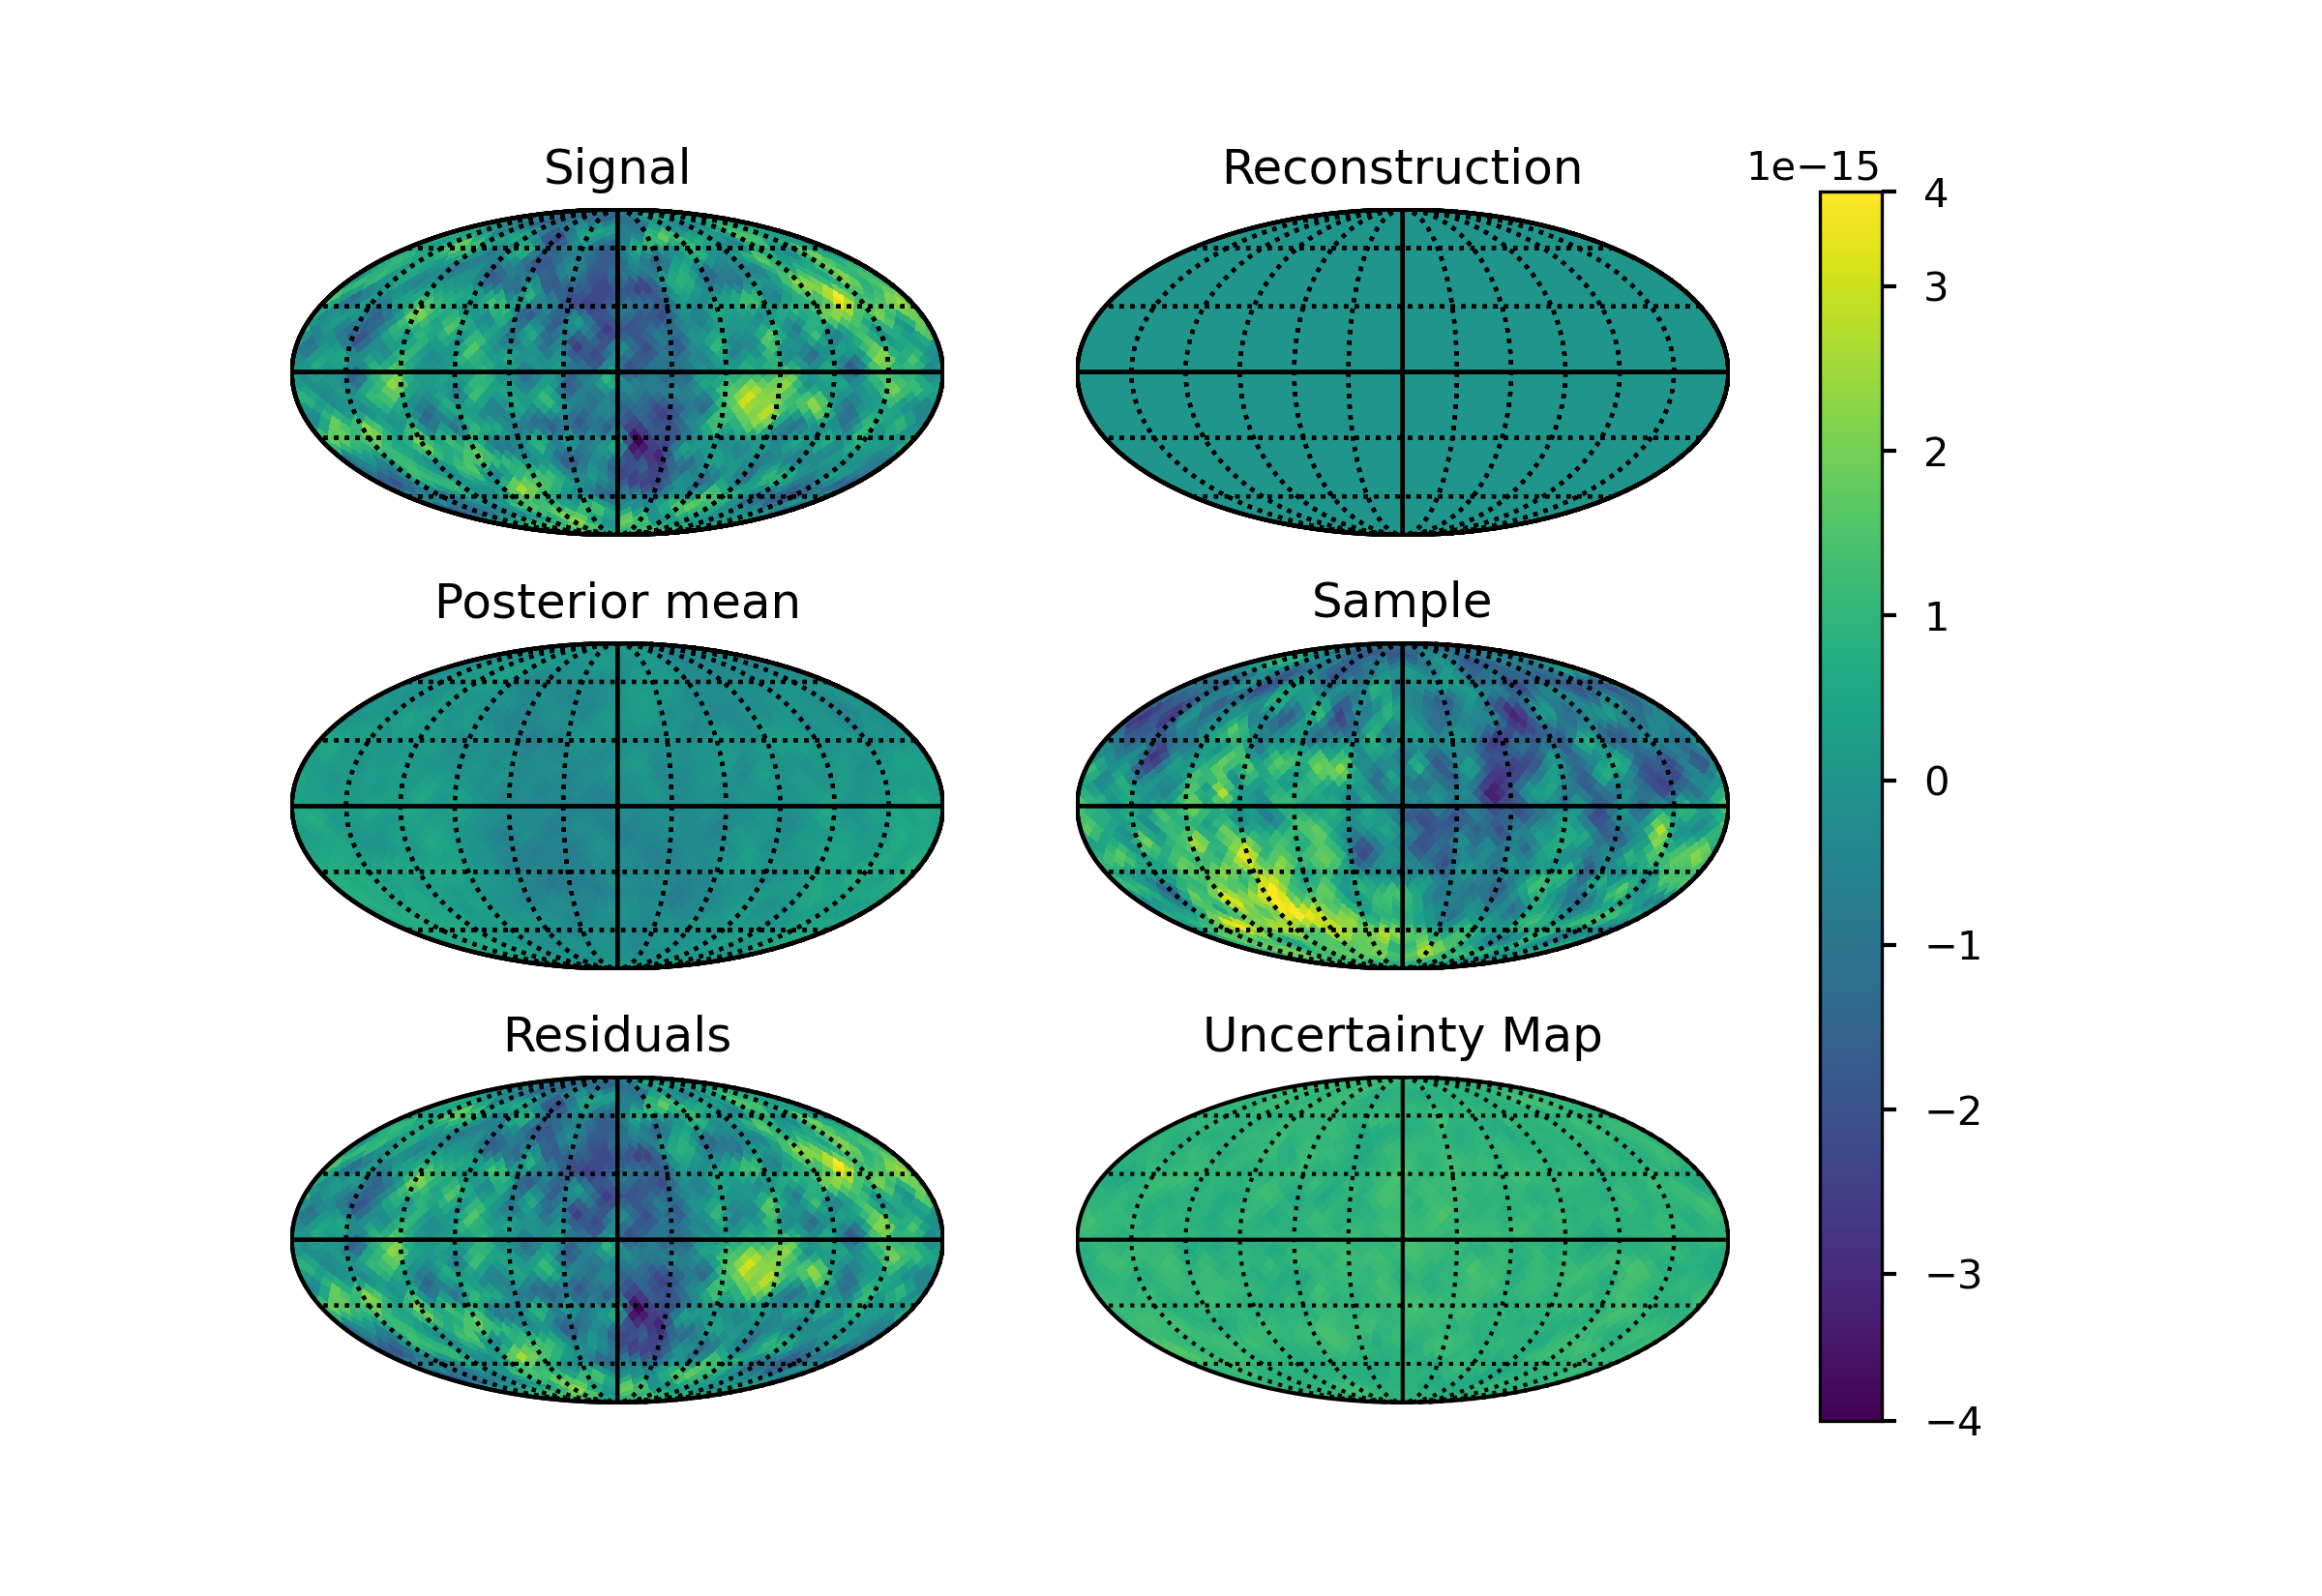
\includegraphics[width=\linewidth]{Images/6plot_cosmo_900Hz_2D.png}}
    \caption{Reconstruction of the CGWB at 900 Hertz on a sky map using the {\tt NIFTy} code. The data on top is generated from the signal which is a realisation of the input power spectrum. The posterior mean is calculated using a Wiener filter. A sample of this is drawn randomly. The residuals represent the difference between signal and reconstruction from the first row. The uncertainty map shows the calculated errors on the reconstruction.}
    \label{sky_maps_cosmo}
\end{figure}

\begin{figure}[h]
    \centering
    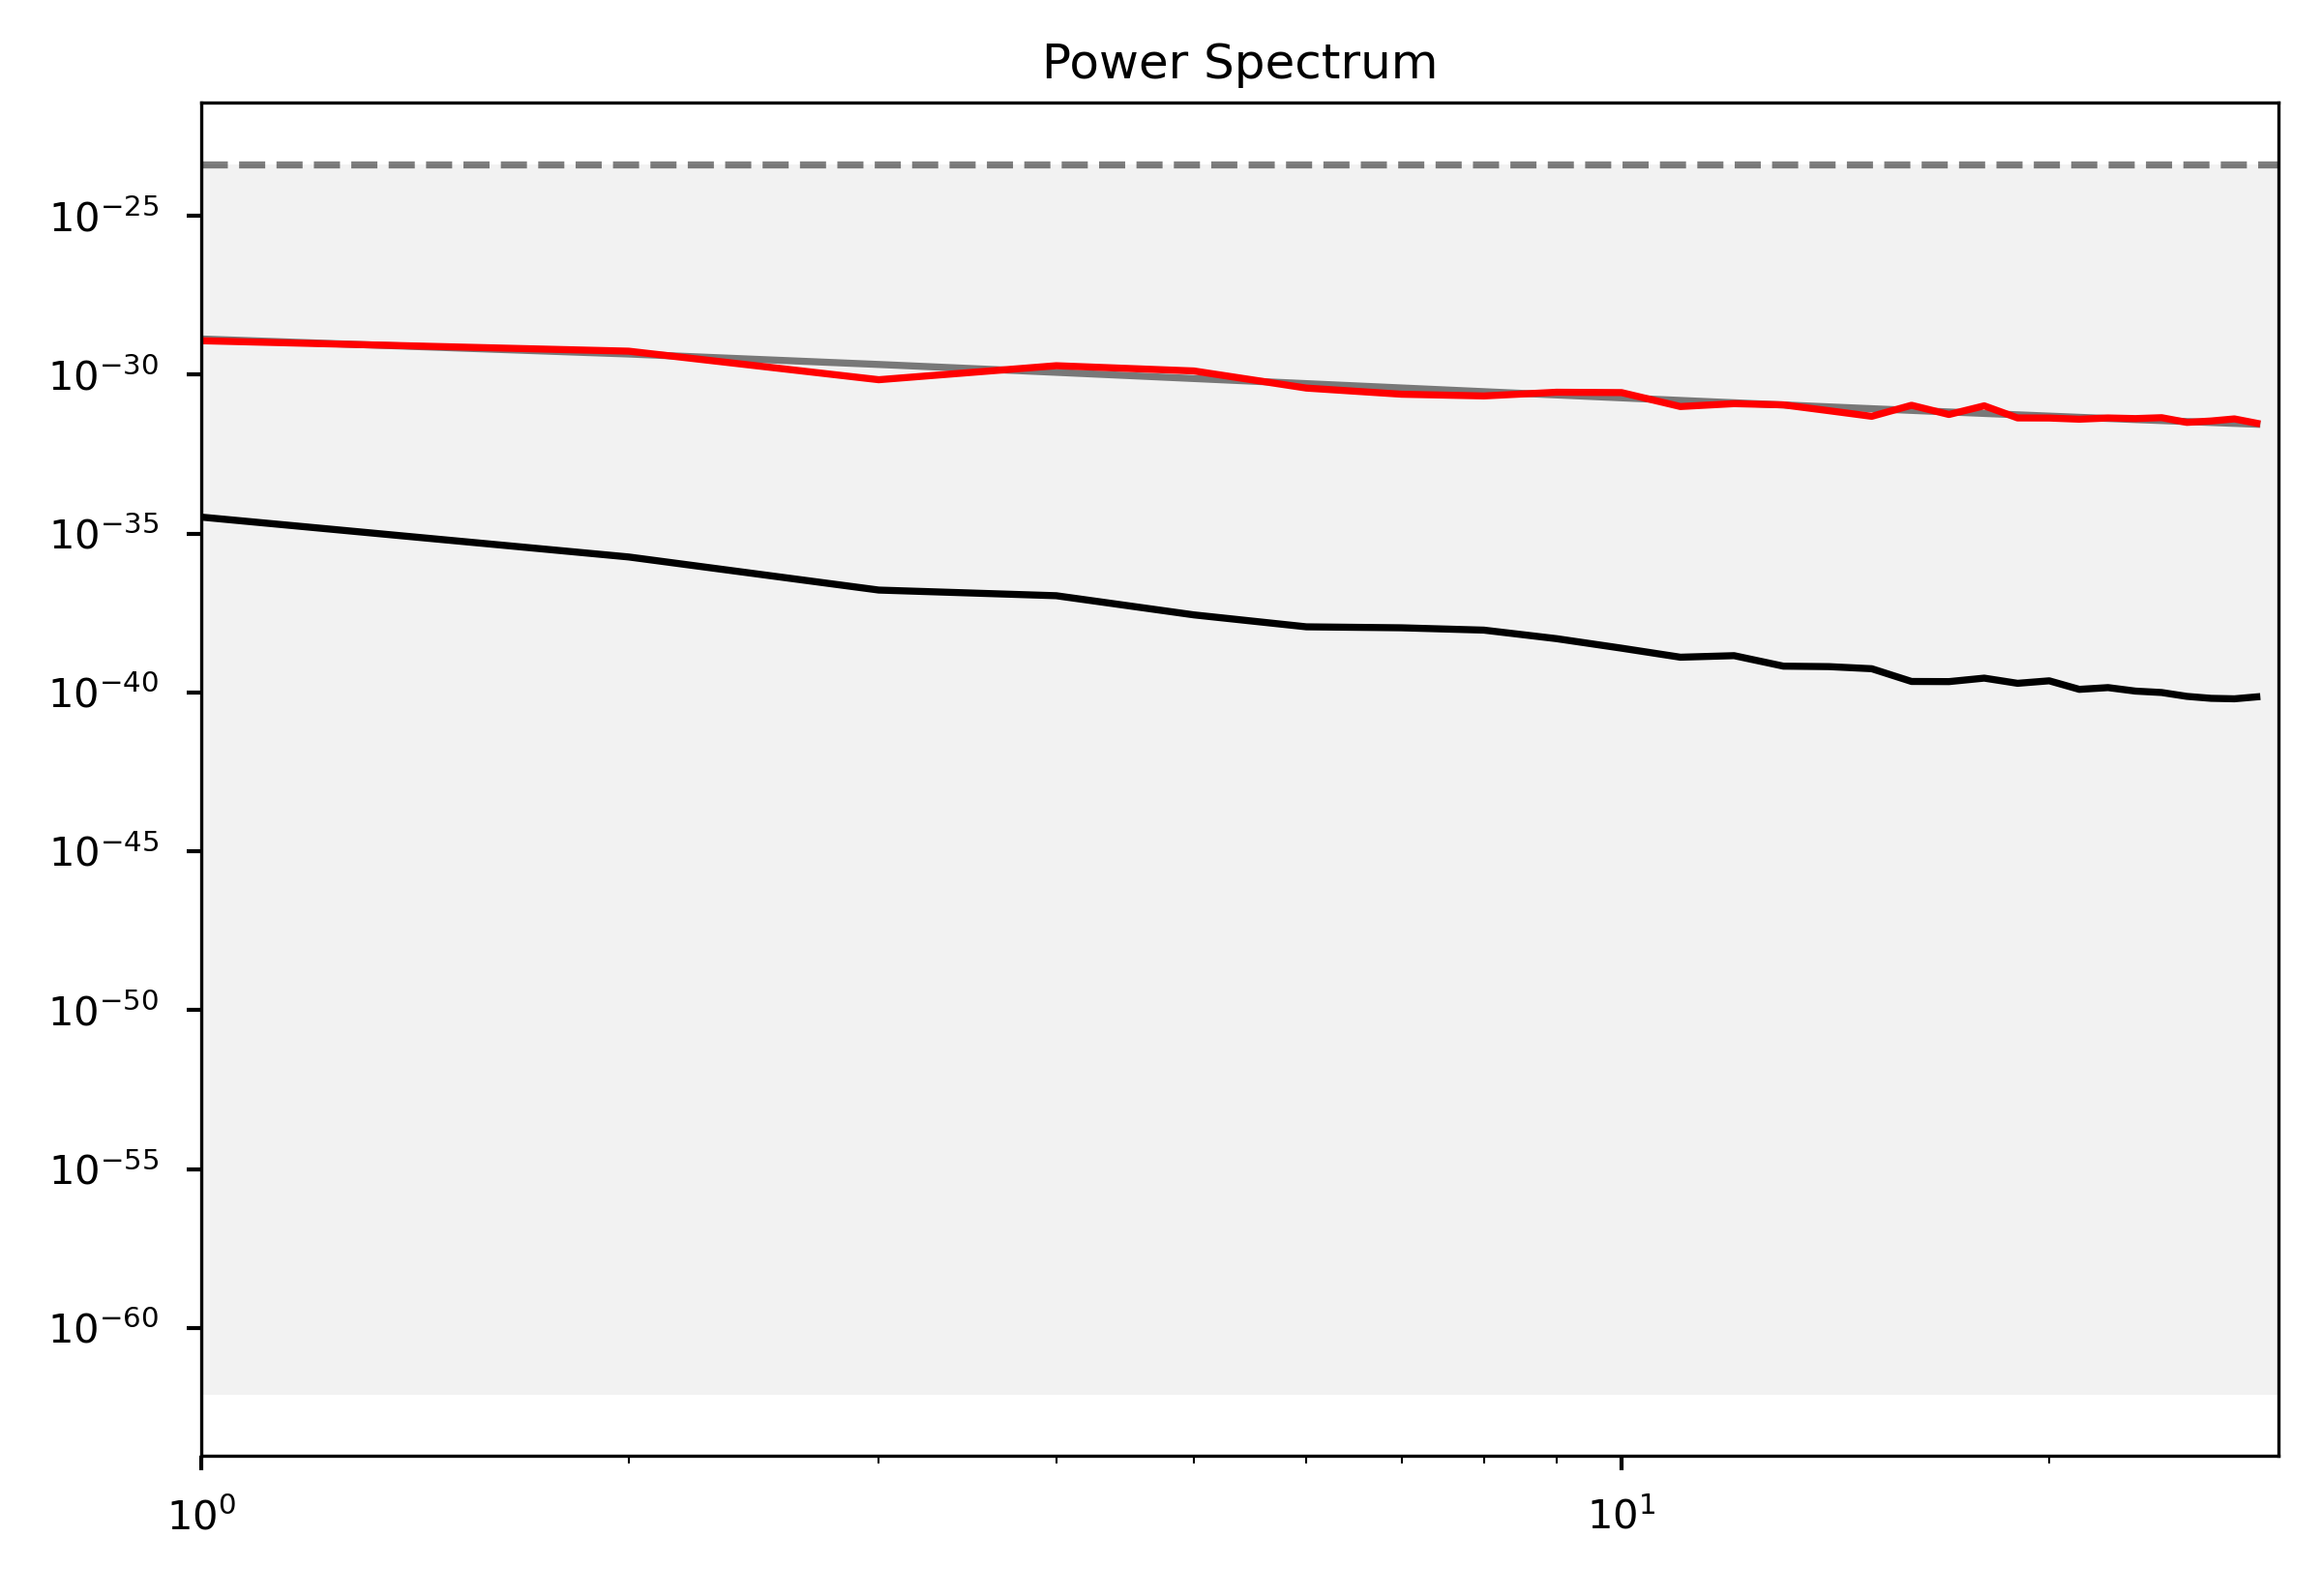
\includegraphics[width=0.8\linewidth]{Images/power_spectrum_cosmo_900Hz_2D.png}
    \caption{The power spectra of the CGWB separation at 900 Hertz. The input power spectrum is shown in grey, the signal realisation in red and the reconstruction using IFT in black.}
    \label{cosmo_power_spectrum_nifty}
\end{figure} 